% Bremen Big Data Challenge - Edition 2019
%
% Data Analysis Competition
%
% Team `gentleman`
%
% Created on March 10, 2019
%
% Authors:
%   Gari Ciodaro <g.ciodaroguerra@jacobs-university.de>
%   Diogo Cosin <d.ayresdeoliveira@jacobs-university.de>
%   Ralph Florent <r.florent@jacobs-university.de>
%
% Contents block for the documentation
%
% 1) Introduction
% 2) Background of the data (data description)
% 3) Data preprocessing
% 4) Data exploitation
% 5) Data Analysis
% 6) Conclusion / Results
% 7) References / Bibliography

% ==============================================================================
% START: Methods, Results, Discussions, Conclusion
% ==============================================================================

\section{Background of the Data}
\subsection{Data Source}

Provided by \emph{"The Bremen Big Data Challenge 2019" Organizers}, the collected data are based on
daily athletic movements \parencite{bbdc}. Using wearable sensors above and below the knee (See
Figure \ref{fig:sensor-placement}) of the individual (athletic), a dataset of 19 individuals, mainly
identified as \emph{subjects}, has been recorded. And as the competition requires, the data of 15
out of the total number of subjects are used as the training dataset and the remaining part as the
testing dataset. The dataset is publicly available online on the official website:
\href{https://bbdc.csl.uni-bremen.de/images/2019/bbdc_2019_Bewegungsdaten_mit_referenz.zip}{BBDC} or
by simply browsing through the following URL: \emph{https://bbdc.csl.uni-bremen.de/index.php/2019h/28-aufgabenstellung-2019}.

\begin{figure}
    \centering
    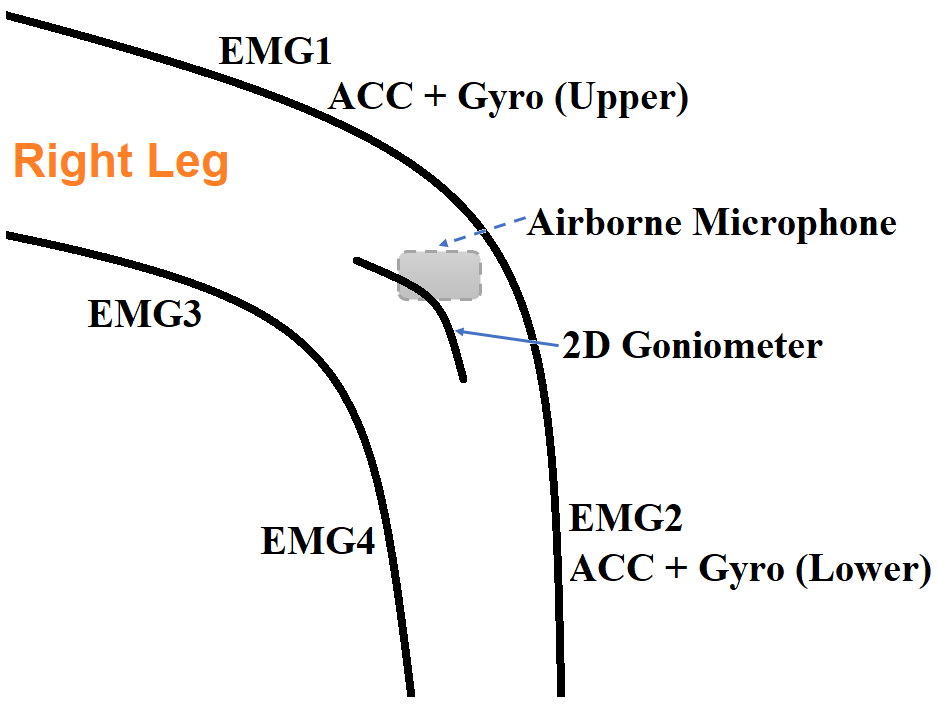
\includegraphics[scale=0.33]{sensor-placement.png}
    \caption{Wearable sensor placement for data measurements. (source: part of the provided data)}
    \label{fig:sensor-placement}
\end{figure}

\subsection{Description and Format}

The data comprise the following 22 movements:
\begin{itemize}
    \item Race ('run')
    \item Walking ('walk')
    \item Standing (standing)
    \item Sitting ('sit')
    \item Get up and sit down ('sit-to-stand', 'stand-to-sit')
    \item Up and down stairs ('stair-up', 'stair-down')
    \item Jump on one or both legs ('jump-one-leg', 'jump-two-leg')
    \item Run left or right ('curve-left-step', 'curve-right-step')
    \item Turn left or right on the spot, left or right foot first ('curve-left-spin-Lfirst',
    'curve-left-spin-Rfirst', 'curve-right-spin-Lfirst', 'curve-right- spin-Rfirst ')
    \item Lateral steps to the left or right ('lateral-shuffle-left', 'lateral-shuffle-right')
    \item Change of direction when running to the right or left, left or right foot first
    ('v-cut-left-left', 'v-cut-left-right', 'v-cut-right-left', 'v-cut' right-Rfirst ')
\end{itemize}

The entire data are available as CSV files, or Comma-Separated Values, and partitioned as training and
testing data, respectively represented by the "\textbf{\emph{train.csv}}" and the "\textbf{\emph{challenge.csv}}"
files. Starting with the training dataset file (\textbf{\emph{train.csv}}), it contains
\emph{UTF-8}\footnote{Unicode Transformation Format, extended ASCII, variable-width encoding.}
character-encoded, line-wise plain texts, whose first line identifies the feature names
followed by the feature values. This file contains a total of 6402 lines, which include both the
feature names and the feature values. The feature names are \textit{Subjects}, \textit{Datafile}, \textit{Label},
and the feature values map respectively each feature name. For instance, the first feature values of
the file are: \textit{Subject02}, \textit{ \path{Subject02 / Subject02_Aufnahme002.csv}},
\textit{stand-to-sit}. Table \ref{table:train-data} illustrates a lightweight version of the
data partition of the training dataset file.

\begin{table}
    \begin{center}
        \begin{tabular}{||c | c | c||}
            \hline % Table headers
            \textbf{Subjects} & \textbf{Datafile} & \textbf{Label} \\ [0.5ex]
            \hline \hline % Table body (row-wise contents)
            Subject02 & \path{Subject02 / Subject02_Aufnahme000.csv} & \textit{curve-left-step} \\
            \hline
            Subject02 & \path{Subject02 / Subject02_Aufnahme001.csv} & \textit{curve-left-step} \\
            \hline
            Subject02 & \path{Subject02 / Subject02_Aufnahme002.csv} & \textit{stand-to-sit} \\
            \hline
            ... & ... & ... \\
            \hline
            Subject19 & \path{Subject19 / Subject19_Aufnahme438.csv} & \textit{curve-right-step} \\
            \hline
            Subject19 & \path{Subject19 / Subject19_Aufnahme439.csv} & \textit{curve-right-spin-Rfirst} \\
            \hline
        \end{tabular}
        \caption{Tabular visualization of the "\textbf{\emph{train.csv}}" dataset}
        \label{table:train-data}
    \end{center}
\end{table}

Similarly, the testing dataset file (\textbf{\emph{challenge.csv}}) is formatted using the same structure
with the exception of the \textit{Label} column, which is unknown and marked with an \emph{X}.
The datafile contains a total of 1739 lines counting both the feature names and feature values.
Table \ref{table:test-data} displays a lightweight version of the data partition of the testing
dataset file.

\begin{table}
    \begin{center}
        \begin{tabular}{||c | c | c||}
            \hline % Table headers
            \textbf{Subjects} & \textbf{Datafile} & \textbf{Label} \\ [0.5ex]
            \hline \hline % Table body (row-wise contents)
            Subject01 & \path{Subject01 / Subject01_Aufnahme000.csv} & \textit{X} \\
            \hline
            Subject01 & \path{Subject01 / Subject01_Aufnahme001.csv} & \textit{X} \\
            \hline
            Subject01 & \path{Subject01 / Subject01_Aufnahme002.csv} & \textit{X} \\
            \hline
            ... & ... & ... \\
            \hline
            Subject15 & \path{Subject15 / Subject15_Aufnahme438.csv} & \textit{X} \\
            \hline
            Subject15 & \path{Subject15 / Subject15_Aufnahme439.csv} & \textit{X} \\
            \hline
        \end{tabular}
        \caption{Tabular visualization of the "\textbf{\emph{challenge.csv}}" dataset}
        \label{table:test-data}
    \end{center}
\end{table}

\noindent
\textbf{Important}: Recalling that the dataset is divided into training and testing data, the subjects
"\emph{Subject01, Subject10, Subject14, Subject15}" are the selected ones that are used as testing
data to assess the solutions. Note the difference in the starting and ending rows of Tables
\ref{table:train-data} and \ref{table:test-data}.

As observed in both Tables \ref{table:train-data} and \ref{table:test-data}, each line corresponds
to a recording of a movement. The columns have the following meanings:
\begin{itemize}
    \item \textbf{\emph{Subject}}: The ID of the subject
    \item \textbf{\emph{Datafile}}: Path of the file containing the sensor data for this recording. For each subject,
    there is a folder in which individual data files contain the sensor data for individual motion
    recordings.
    \item \textbf{\emph{Label}}: The movement that was recorded
\end{itemize}

Particularly, the \emph{Label} column of the testing dataset contains repeatedly the letter "\textit{X}"
to indicate that this value is not present. That is, at the time of submitting solutions, the submission should
exactly match the testing data, where each \emph{X} will be replaced by a label. This label corresponds to the
classification result of a specific movement. It is important that the spelling (including upper / lower
case) of the textual labels matches exactly the spelling of the labels in the training data.

As mentioned above, the datafiles are references to other CSV files. For example, the path file
\path{Subject02 / Subject02_Aufnahme000.csv} is a CSV file itself within a folder named \emph{Subject02}
located in the root path (i.e., the current directory of the downloaded zip files). The CSV file itself
is dataset with a proper format. Basically, the file has a set of comma-separated numbered-values
that looks like this: \textit{32688,32224,32991,32609,32790,33048,37168,34610,27374,29068,29264,
28408,31784,28133,29295,29244,33216,37140,34736}.

Each line represents the sensor values measured at one time (sampled at 1000 Hz). The columns
represent the individual wearable sensors recording the human activities (see Figure \ref{fig:sensor-placement}):

\begin{enumerate}
    \item EMG1
    \item EMG2
    \item EMG3
    \item EMG4
    \item Airborne
    \item ACC upper X
    \item ACC upper Y
    \item ACC upper Z
    \item Goniometer X
    \item ACC lower X
    \item ACC lower Y
    \item ACC lower Z
    \item Goniometer Y
    \item Gyro upper X
    \item Gyro upper Y
    \item Gyro upper Z
    \item Gyro lower X
    \item Gyro lower Y
    \item Gyro lower Z
\end{enumerate}

% source is needed
The size of the CSV datafiles vary inappropriately. That is, in most cases, due to inaccurate measurements,
random initialization states, mechanical flaws, computational and processing cost, and so on.


\section{General comments}

\subsection{Notation}
Let us defined a modeling procedure as  a function $\mathcal{P}(\Theta): \mathbb{R}^{m} \longrightarrow \mathbb{R}^{k}$ where $m$ is the number of features, $k$ is the number of classes, and $\Theta : \{Preprocessing_{method}, Feature_{extration}, Statistical_{Tecnique} \}$ is a set representing parameters. Giving this abstraction $\Theta$ modifies the structure  $\mathcal{P}$ but always takes a \textit{feature vector} $X \in  \mathbb{R}^{m}$, and returns a \textit{Probability vector} $Y \in  \mathbb{R}^{k}$ where each component $\in  [0,1]$.\\

It is clear that the $\mathcal{P}(\Theta)$ that represents exactly the reality regarding athletics movements is unknown to us, which let us to defined a measure of the amount of veracity that a giving $\mathcal{P}$ has compare to reality. 

\begin{equation}
accuracy=  \frac{\sum Correct_{classification}}{N}
\end{equation}

\subsection{Cross validation}

\textit{Guys please explain here what cv is, why is important to use, that is what is the shit with variance and bias, why overfit may occurs. In general terms. why is a good stimator of the test error over unseen data.}

\subsection{Curse of dimensionality}

\textit{Guys please explain this also. remember to say the 10 feature rule thumbs and cited jaeger lectures notes.}


\section{Data Preprocessing}

Two \textit{Preprocessing methods} procedures were implemented.

\textbf{Preprocessing method 1}:
\begin{enumerate}
	\item Take a \textbf{subject file}(each file contains a class movement). It can be viewed as $[19 \times N_{fr}]$ matrix composed by 19 columns vectors $S_{data} \in \mathbb{R}^{N_{fr} \times 1}$  where number of records in file is $N_{fr} \in \mathbb{N}^{>0}$.
	\item Transpose each $S_{data}$ into a row vector, concatenating them into one single vector $S_{concat} \in  \mathbb{R}^{1 \times 19*N_{fr} }$ 
	\item Repeat step 1 and 2 for every subject file.
	\item Create a dataset with the rows of step 3 with it according it corresponding label (extracted from the name of the file). This data set is a matrix $D$ of dimensions $[6401 \times (19*N_{fr})]$. For $N_{fr}=56810$ $D$ is $[6401 \times 1079390+1]$.
\end{enumerate}

\textbf{Preprocessing method 2}:
\begin{enumerate}
	\item Take a \textbf{subject file}(each file contains a class movement). It can be viewed as $[19 \times N_{fr}]$ matrix composed by 19 columns vectors $S_{data} \in \mathbb{R}^{N_{fr} \times 1}$  where number of records in file is $N_{fr} \in \mathbb{N}^{>0}$.
	\item For each $S_{data}$ decomposed it as $s_{data}=\mu+\omega$ where $\mu$ is a smoothed version of $s_{data}$ calculated using lowess with tree points average weighted linear regression. A complete derivation of this algorithm can be found in \cite{1}. Having $s_{data}$ and $\mu$ calculate $\omega =s_{data}-\mu$. Create a vector $\mu_{sta} \in \mathbb{R}^{3}$ with first tree statistical moments of $\mu$, that is, the average, the variance, and the steepness. calculate the discrete Fourier transformation of $\omega$, extract the first five coefficients and put them in a vector $\omega_{fft} \in \mathbb{R}^{5}$. A complete derivation of this algorithms can be found in \cite{2}.
	take $\mu_{sta}$ and concatenate it with $\omega_{fft}$ into a row vector $S \in \mathbb{R}^{8}$
	\item concatenate each $S$ into a single vector $S_{row} \in \mathbb{R}^{8*19}$
	\item Repeat steps 1 to 3 for every \textbf{subject file} and stack the vectors $S$ with its corresponding label into a matrix $D$ is $[6401 \times 8*19]$.
\end{enumerate}

 For $Preprocessing_{ \ method \ 1}$ the parameter $N_{fr}$ had to be set, since each \textbf{subject file} had different number records. By observing a 100 random sample of files, we concluded rather arbitrarily that  $N_{fr}=56810$  was reasonable number of records. In case a particular file did not meet this requirement, the signal per sensor would repeat itself until the desired $N_{fr}$ was reached. The idea with $Preprocessing_{ \ method \ 2}$ was to capture the general properties of the movement(using $\mu_{sta}$) in terms of its statistical moments. On the other hand, we also attempted to capture information about the periodicity of the movement using $\omega_{fft}$. 


\section{Data Exploitation}

Depending on the $Preprocessing_{method}$ some $Feature_{extration}$ and $Statistical_{Tecnique}$ combination would more adequate to implement than other. Here we only present highest \textit{accuracy} combinations. 

\subsection{Data Exploitation with $Preprocessing_{ \ method \ 1}$}

One problem that is immediately observed with $Preprocessing_{ \ method \ 1}$ is the immense dimensionality of the sample space, therefore trying to find a $Statistical_{Tecnique}$  capable of learning an adequate decision function is basically impossible. To bypass this problem implemented a $Feature_{extration}$ and $Statistical_{Tecnique}$ shown in the Figure \ref{dig:p1}.


\begin{figure}[htpb!]
	\centering 
	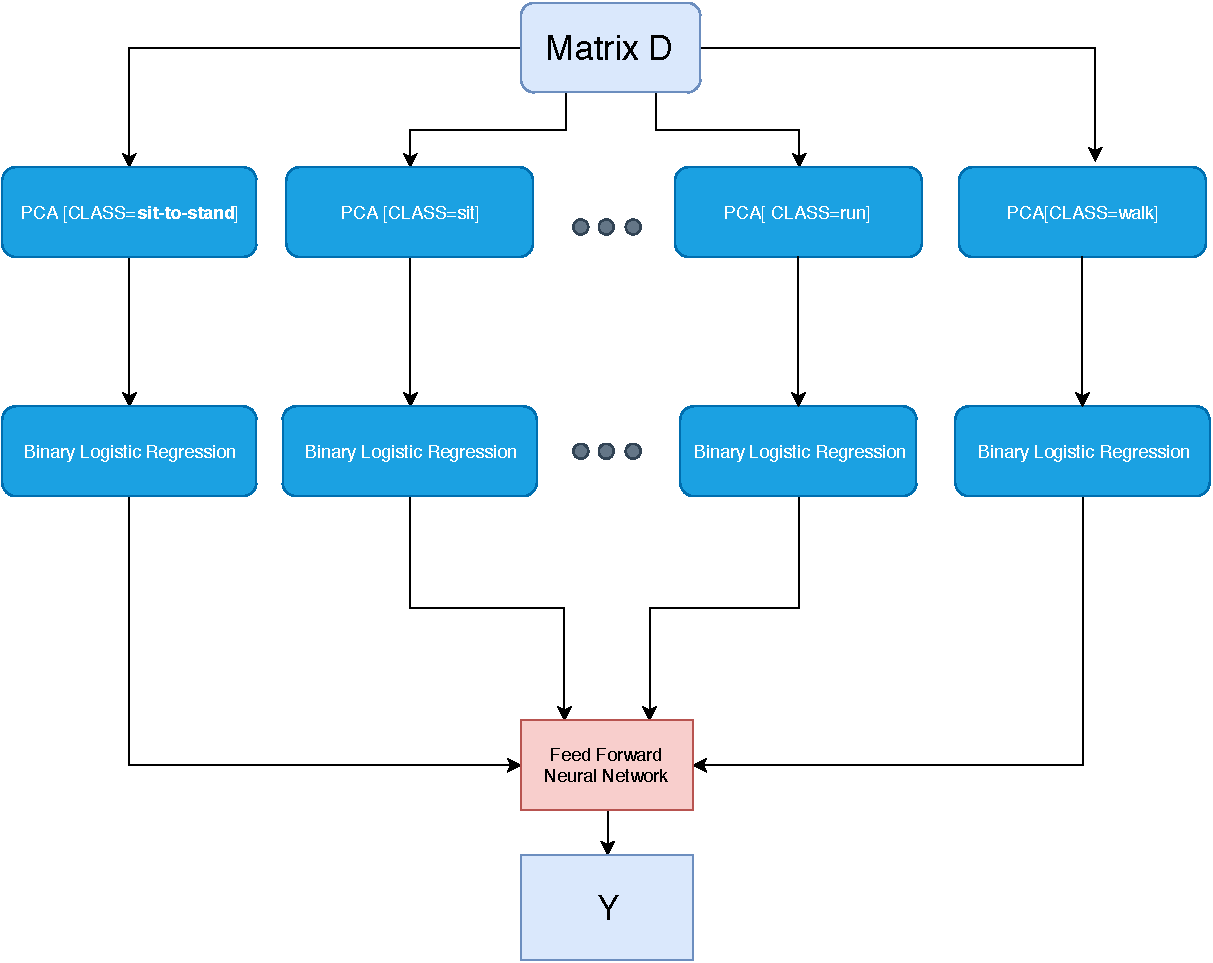
\includegraphics[width=0.7\textwidth]{images/scheme_1.pdf}
	\caption{$\mathcal{P}(\Theta_{1})$  Scheme} 
	\label{dig:p1} 
\end{figure}

We theorized that the importance of features in matrix $D$ measured by its variance will strongly depend on the particular movement involved, acknowledging this we filtered matrix $D$ by class, and applied principal component analysis $PCA_{|class}: \mathbb{R}^{1079390} \longrightarrow \mathbb{R}^{275}$ to extract the first 275 principal components(this transformation will be the beginning a branch in Figure \ref{dig:p1}) that accounts to 90 $\%$ of the variance. Note that the first level in \ref{dig:p1} has 22 $PCA_{|class}$ extractors. For training, matrix $D$ is passed without filtering per label to each $PCA_{|class}$ and then feed to a \textit{Binary logistic regression} $LogR_{|class}: \mathbb{R}^{275} \longrightarrow [0,1]$ where the classes are encoded in \textit{one vs all} manner. Each of the $LogR_{|class}$ will output a degree of believe that a particular $X$ belows to a class $k$. Finally concatenating the degree of believe predicted by each $LogR_{|class}$ we construct a $X' \in \mathbb{R}^{22}$. Finally $X'$ is passed to a single feed forward neuronal network $NN: \mathbb{R}^{22} \longrightarrow  \mathbb{R}^{22} $ that predicts our final probability vector $Y$ in a \textit{hot encoded} structure, we take the maximum component and assign its corresponding label to that register.


\begin{equation}
\Theta_{1}:= \{ Preprocessing_{ \ method \ 1},PCA_{|class},LogR_{|class},NN \}
\label{eq:1}
\end{equation}


\subsection{Data Exploitation with $Preprocessing_{ \ method \ 2}$}
The dimension of $X$ using $Preprocessing_{ \ method \ 2}$ is $R^{152}$ so no further dimension reduction is required. We implemented a variety of feed forward neuron networks using tensor flow, where we varied the Network architecture composed by the number of hidden units $H_{units} \in \mathbb{N}^{>0}$ per hidden layer $H_{L} \in \mathbb{N}^{>0}$ the regularization parameter $\alpha \in \mathbb{R}^{>0}$, and the activation functions, namely $ \{  Logistic, tanh, relu \}$. From Figures \ref{sm1} to  \ref{sm22} we can observe $\mu$ signal examples per label.

\begin{equation}
\Theta_{2}:= \{ Preprocessing_{ \ method \ 2},NN \}
\label{eq:2}
\end{equation}


\begin{figure}[!tbp]
	\begin{minipage}[b]{0.31\textwidth}
		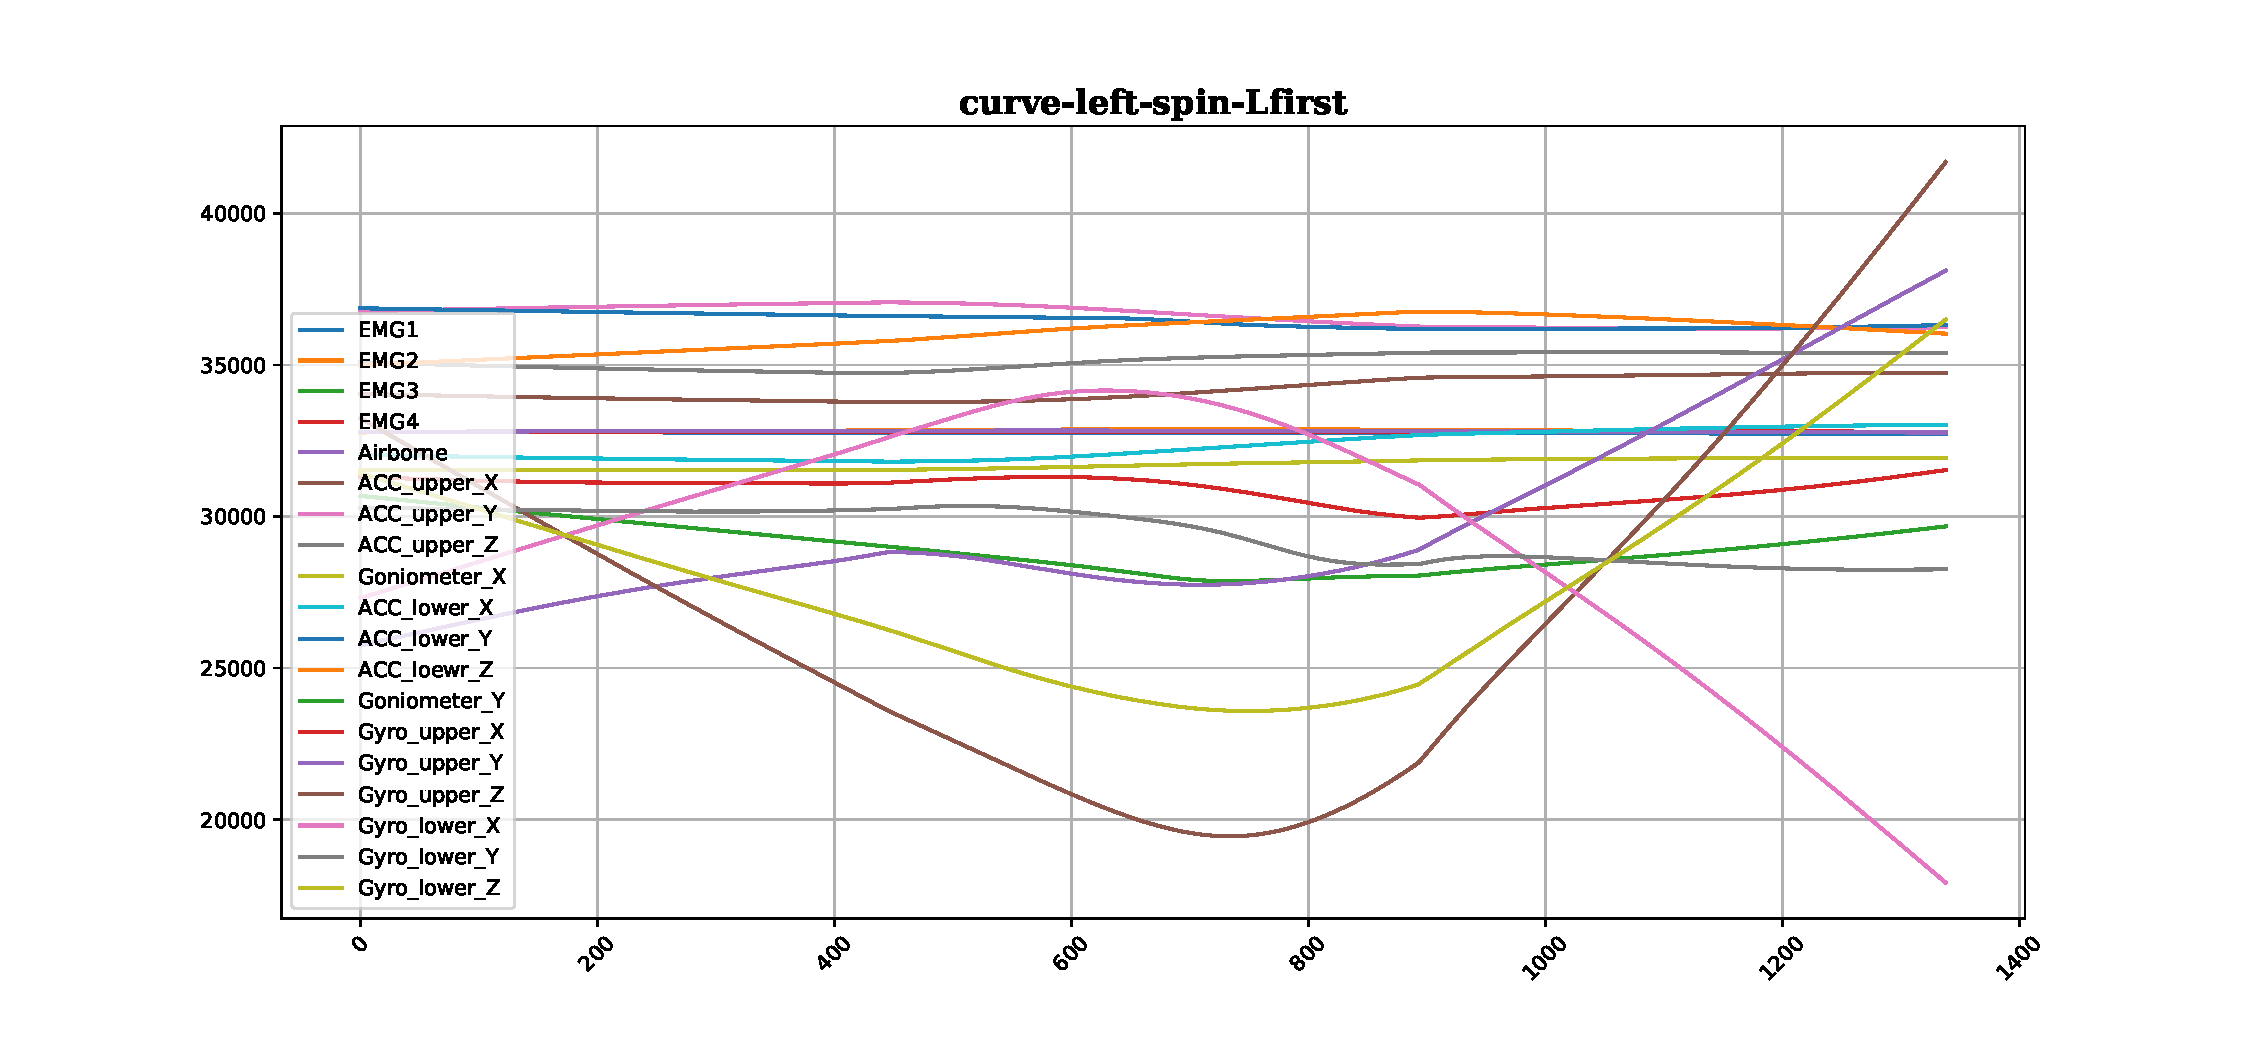
\includegraphics[width=\textwidth]{images/curve-left-spin-Lfirst_example.pdf}
		\caption{curve-left-spin-Lfirst}
		\label{sm1}
	\end{minipage}
	\begin{minipage}[b]{0.31\textwidth}
		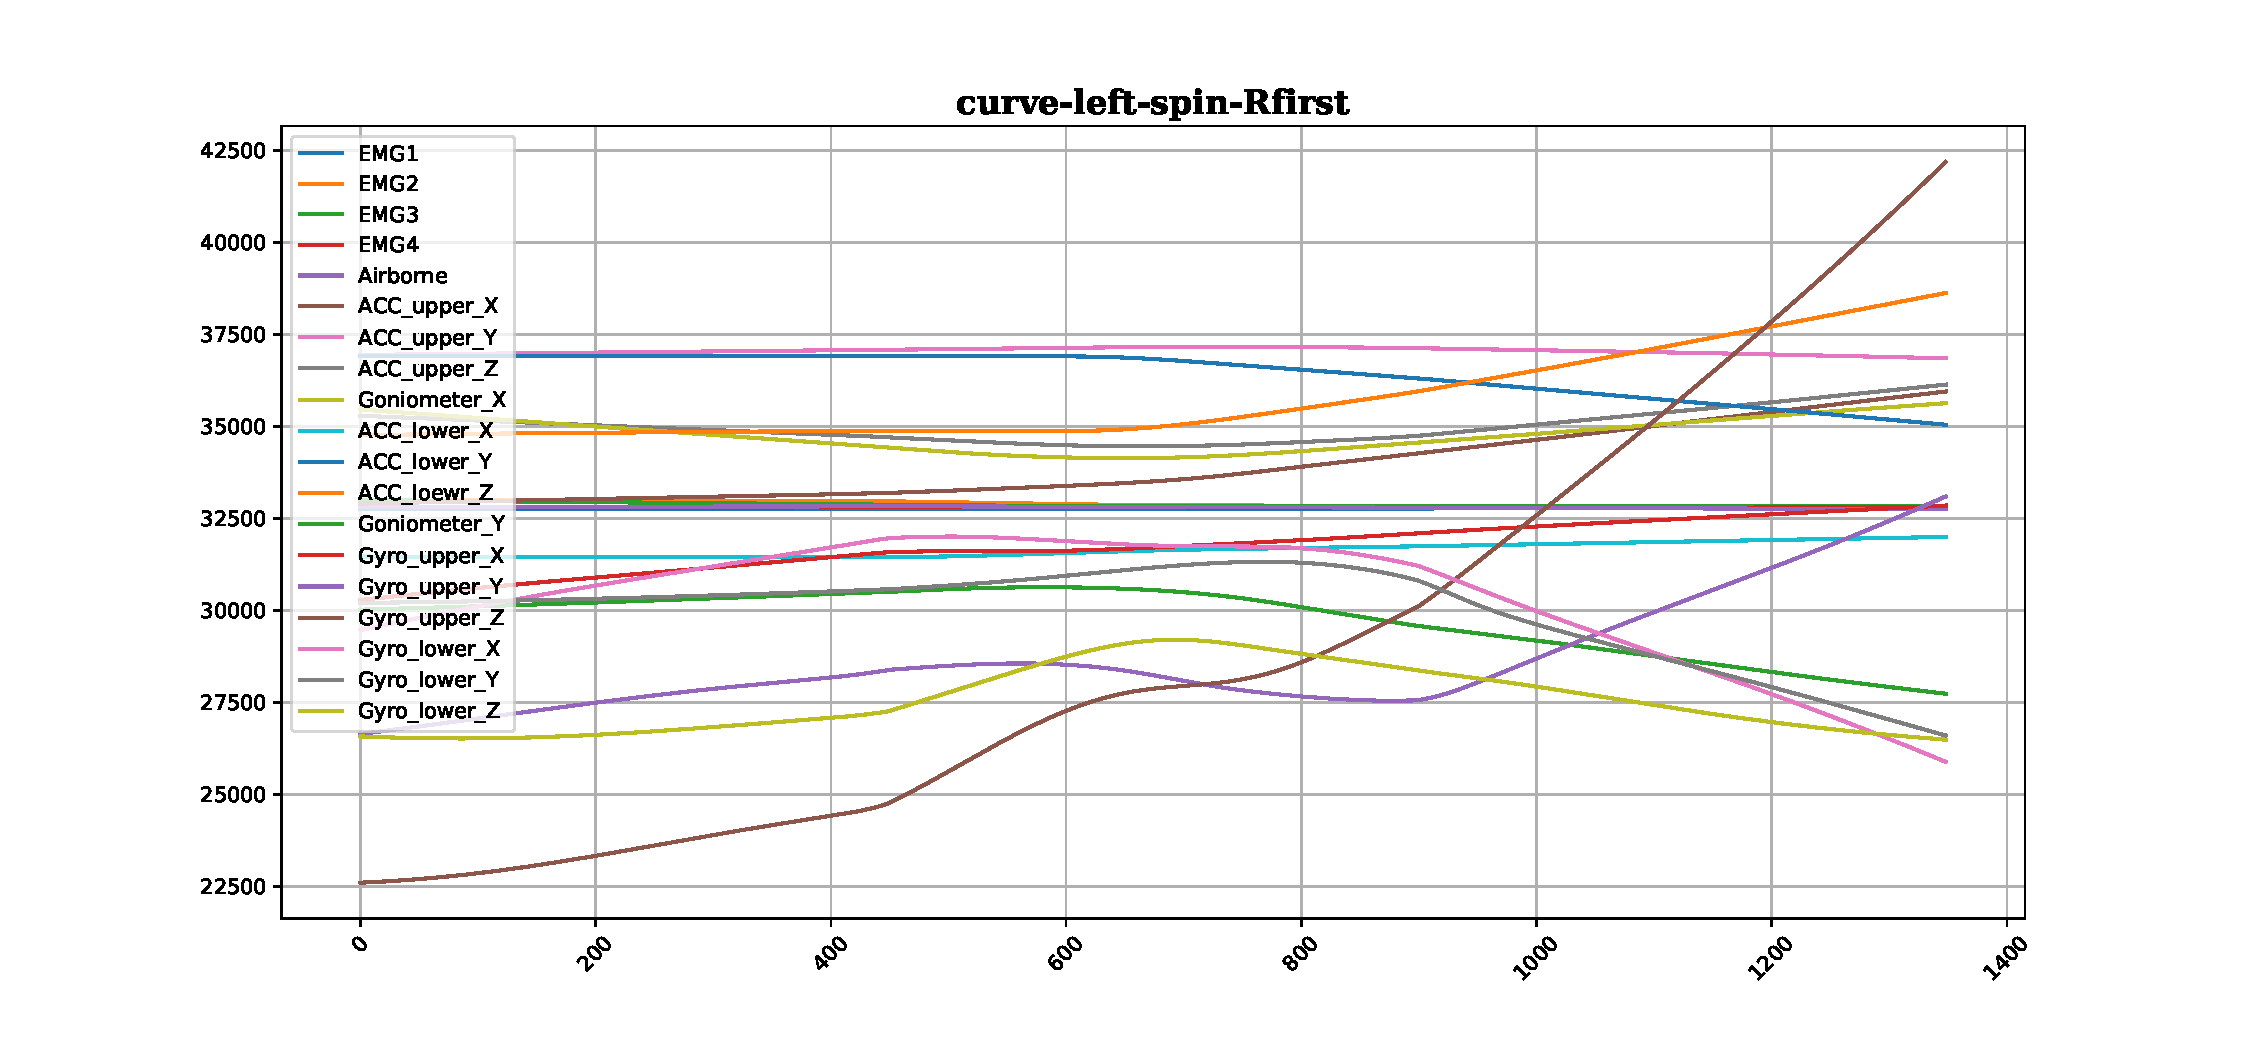
\includegraphics[width=\textwidth]{images/curve-left-spin-Rfirst_example.pdf}
		\caption{curve-left-spin-Rfirst}
	\end{minipage}
	\begin{minipage}[b]{0.31\textwidth}
		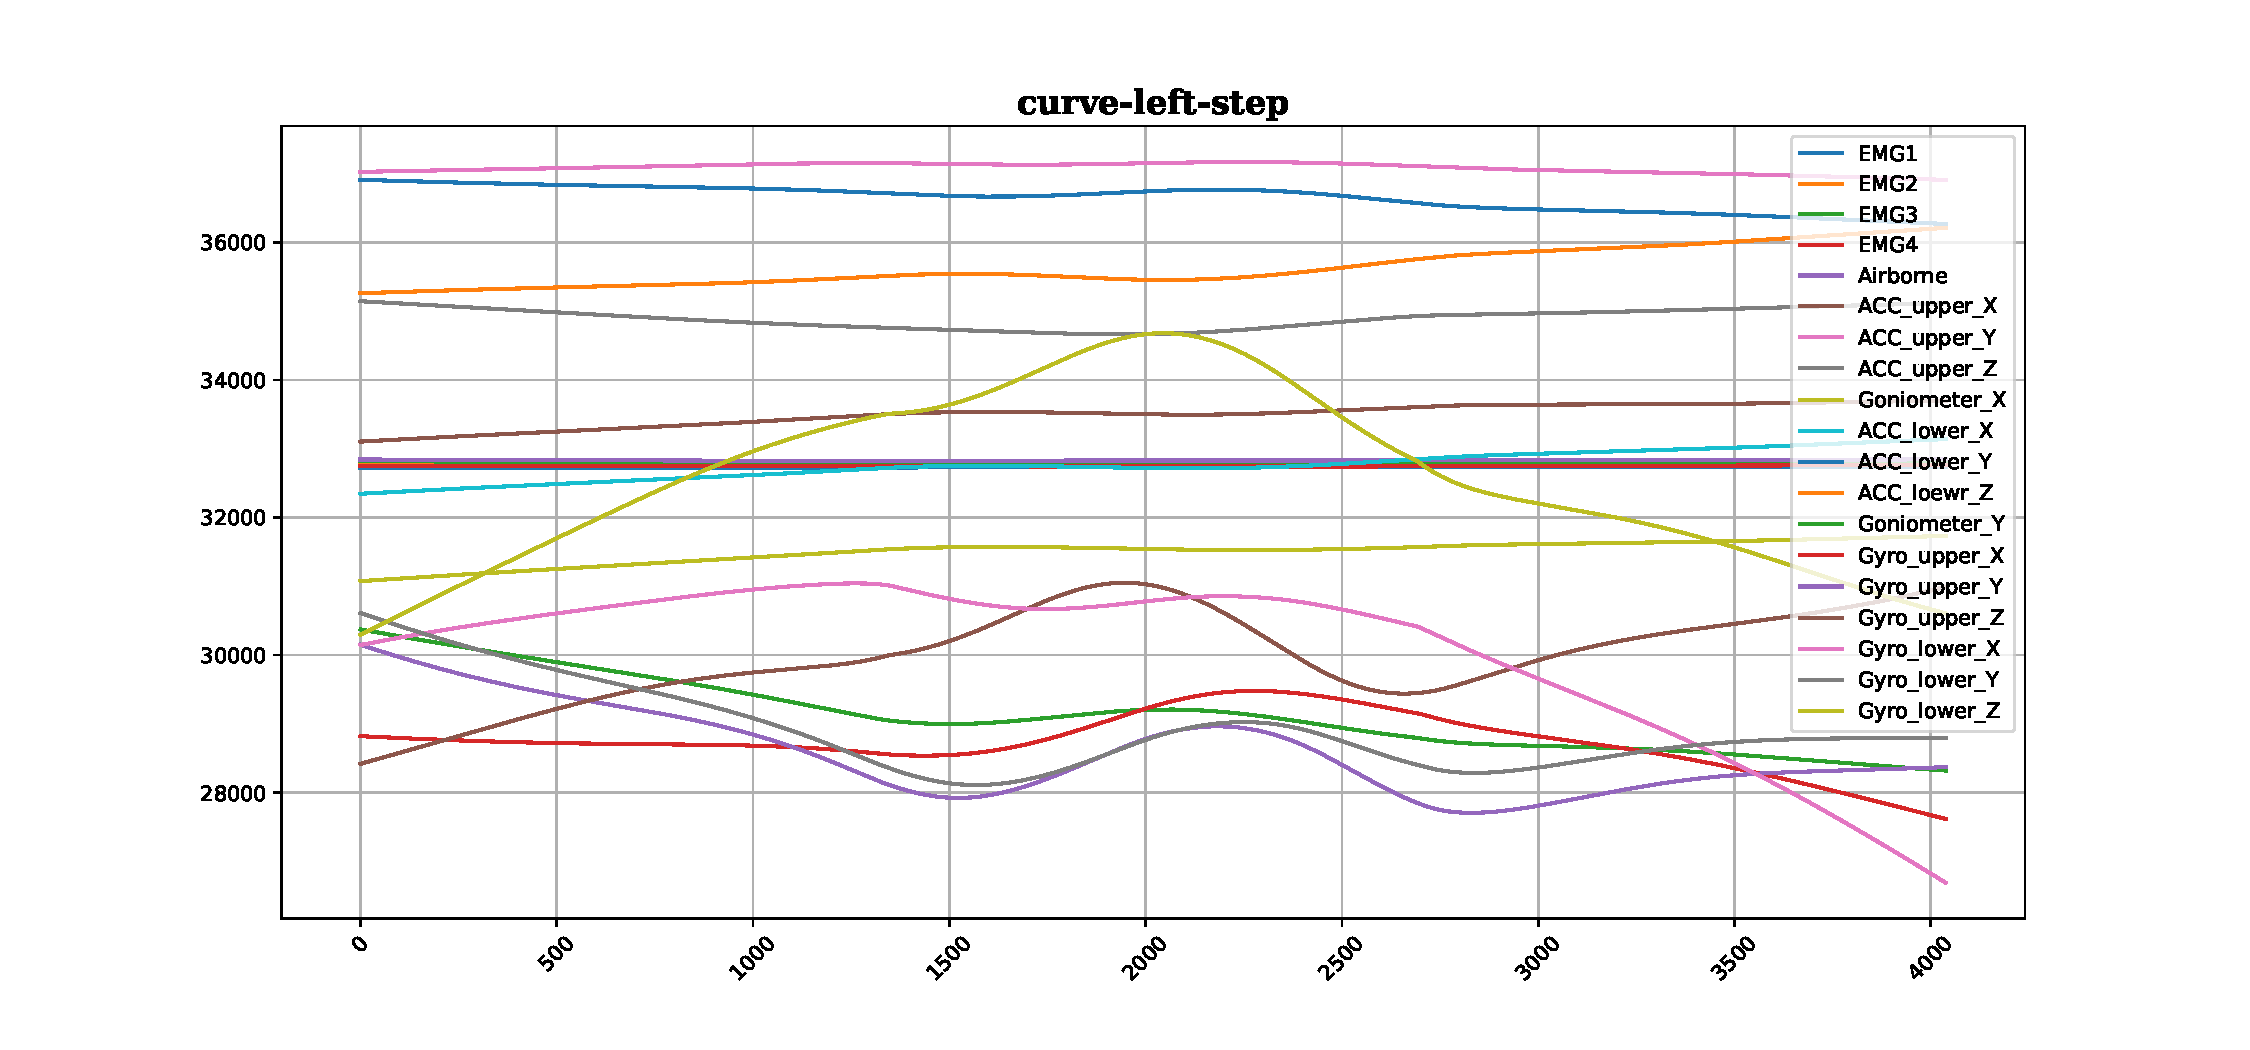
\includegraphics[width=\textwidth]{images/curve-left-step_example.pdf}
		\caption{curve-left-step}
	\end{minipage}
\end{figure}

\begin{figure}[!tbp]
	\begin{minipage}[b]{0.31\textwidth}
		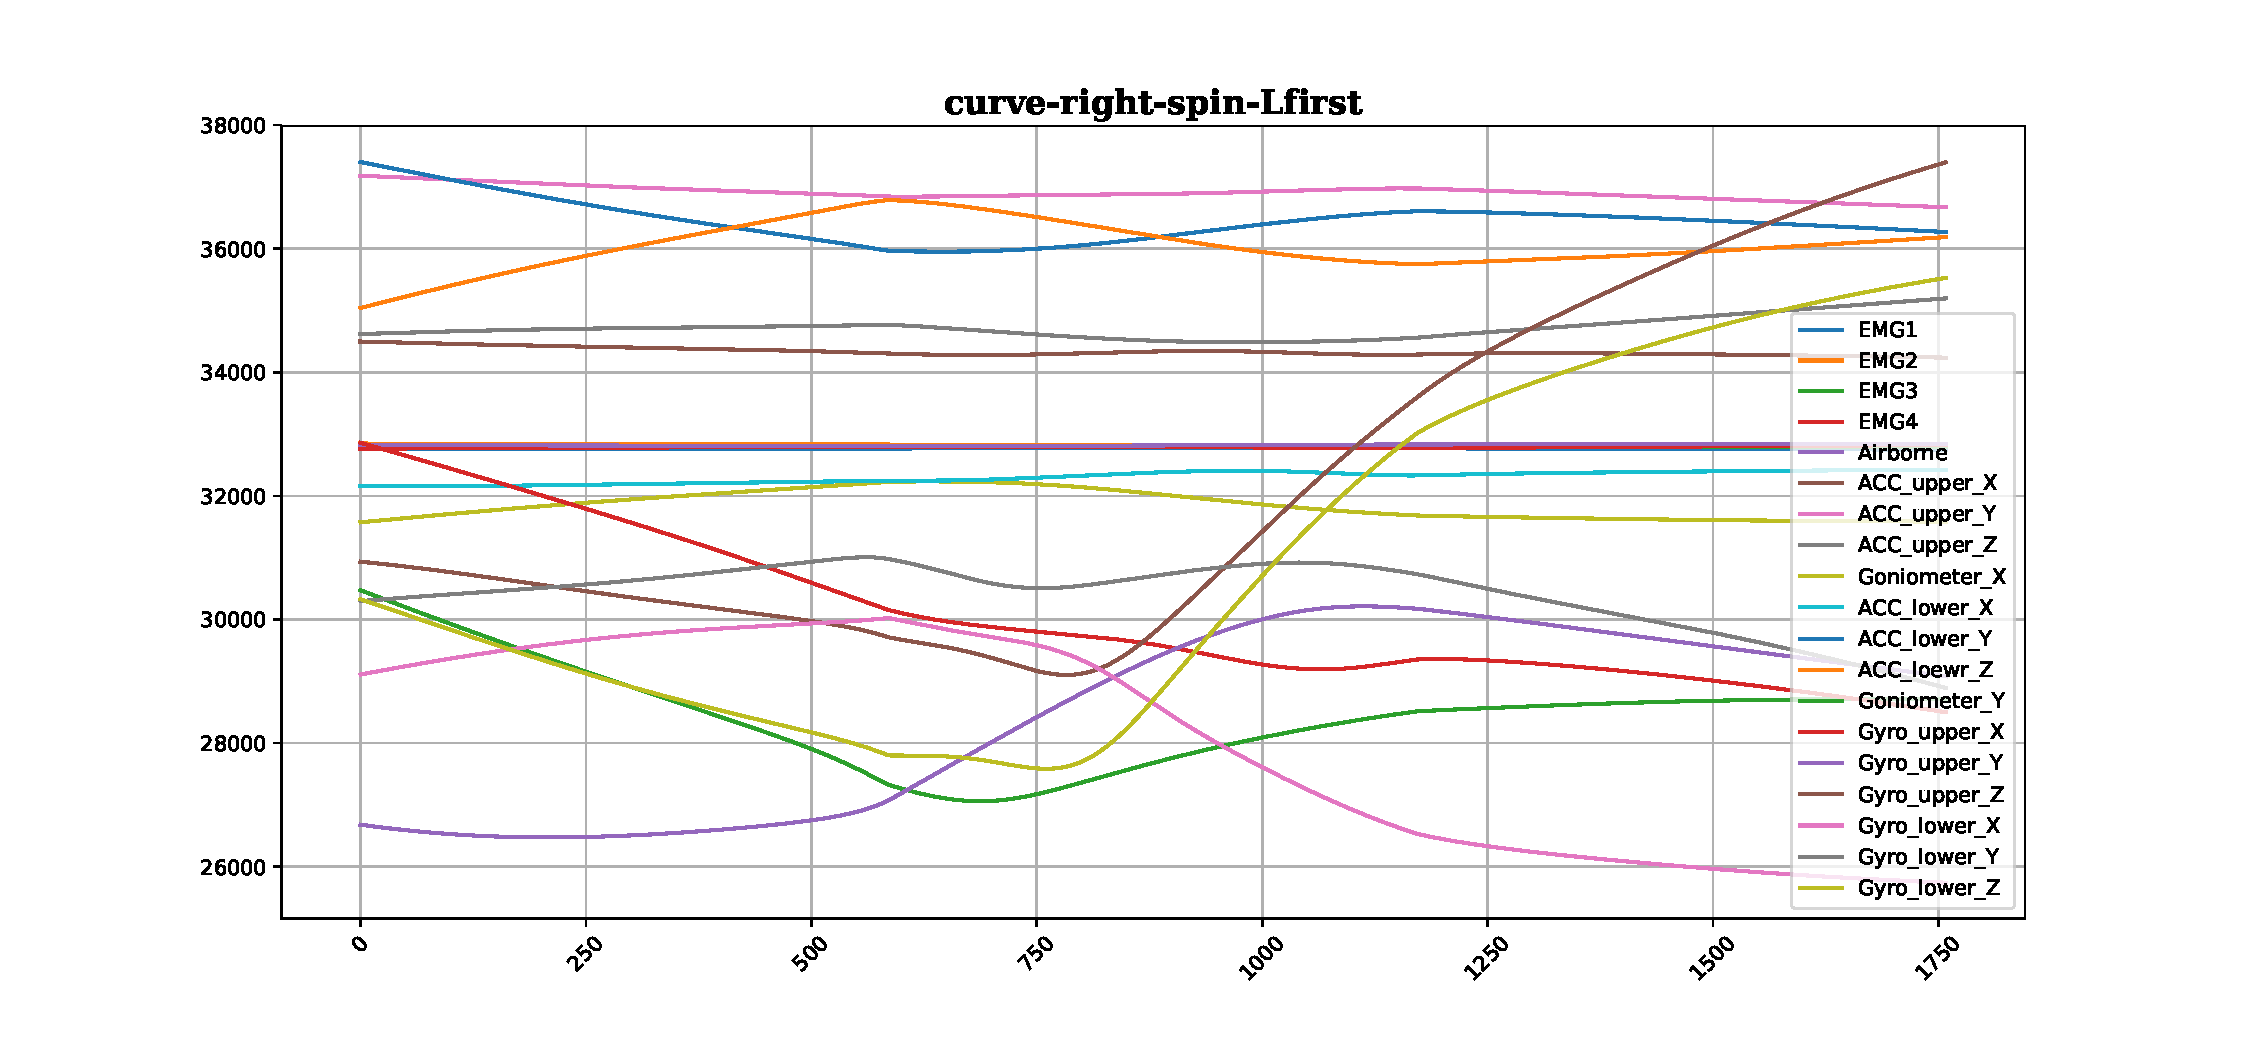
\includegraphics[width=\textwidth]{images/curve-right-spin-Lfirst_example.pdf}
		\caption{curRight-spin-Lfirst}
	\end{minipage}
	\begin{minipage}[b]{0.31\textwidth}
		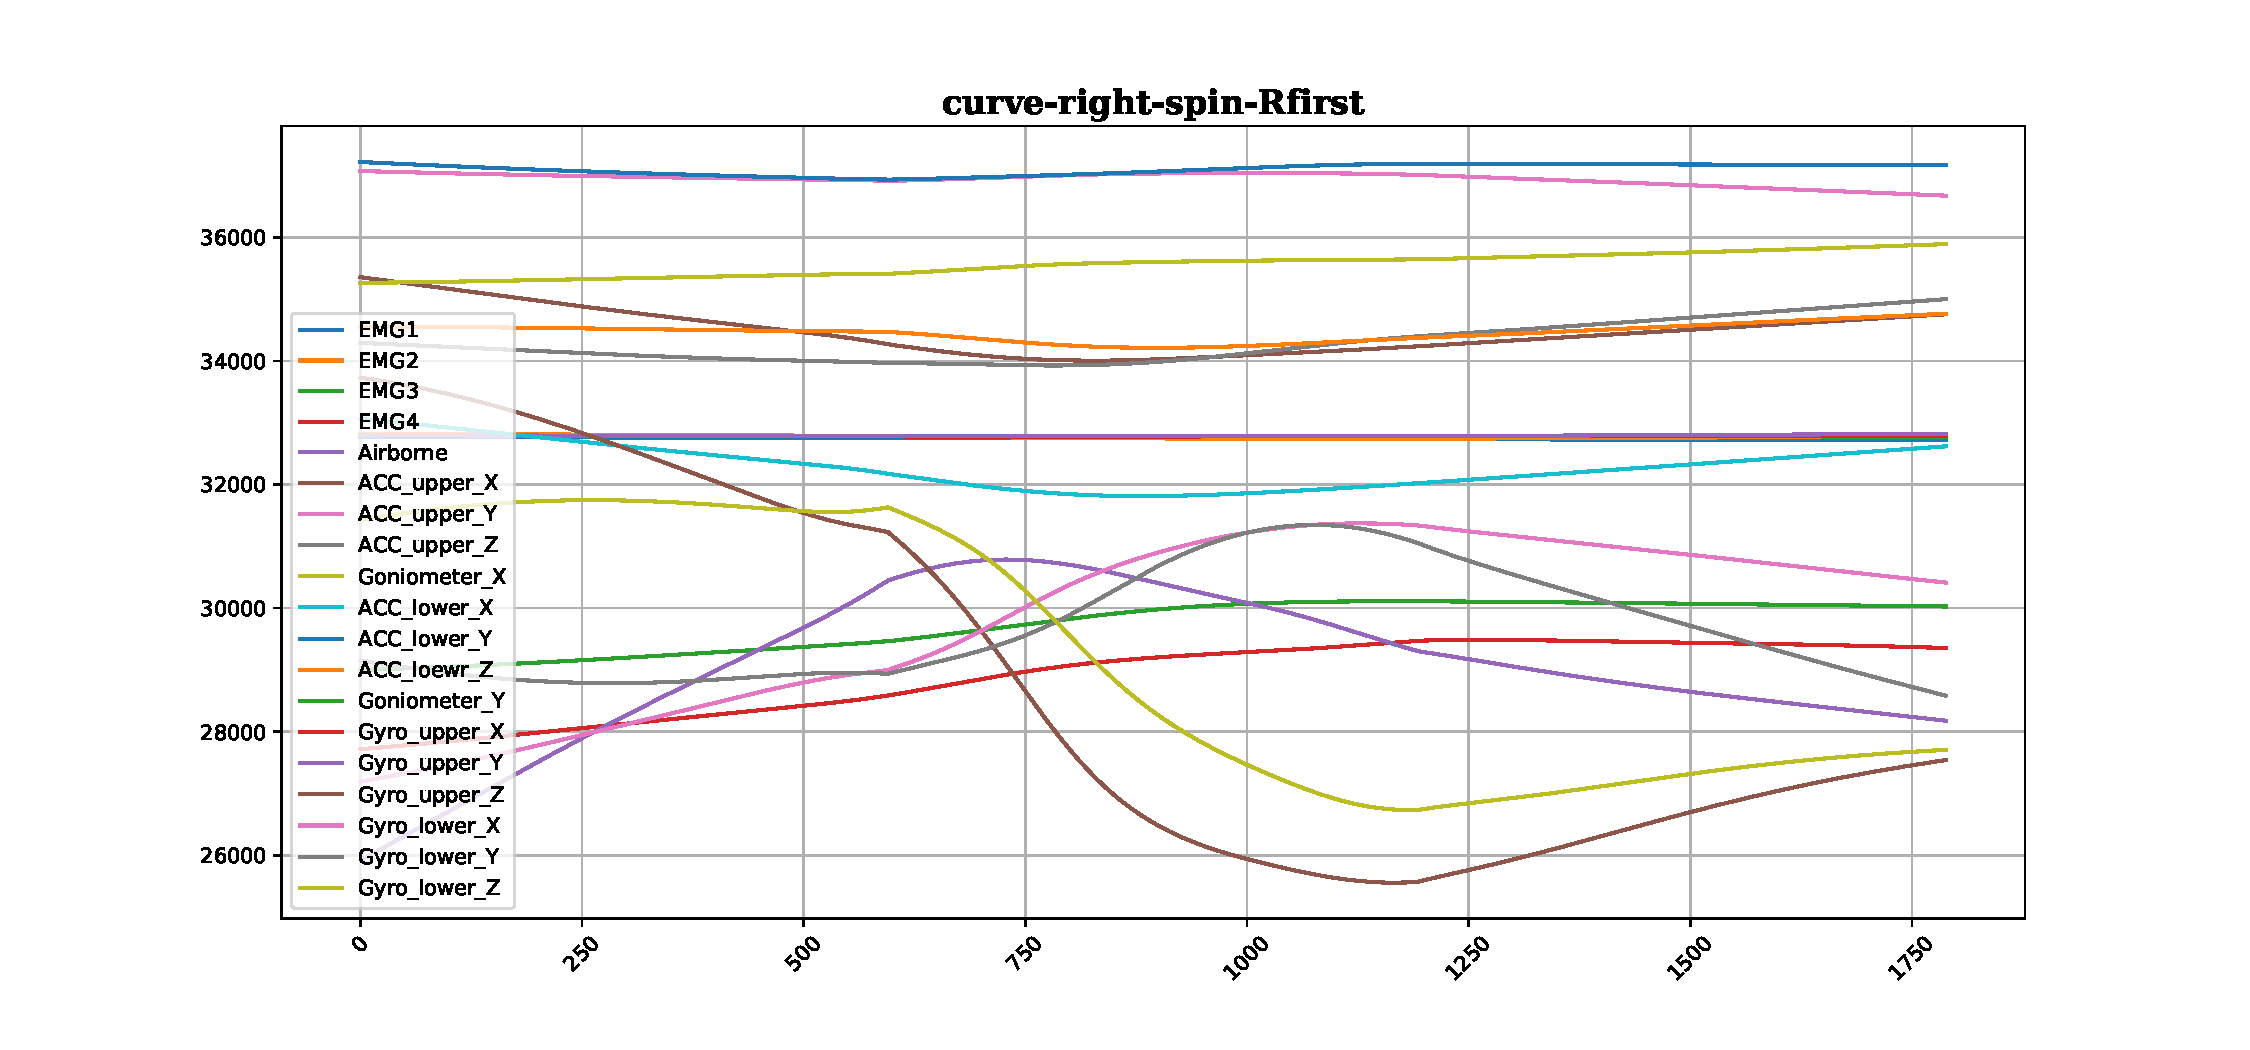
\includegraphics[width=\textwidth]{images/curve-right-spin-Rfirst_example.pdf}
		\caption{curRight-spin-Rfirst}
	\end{minipage}
	\begin{minipage}[b]{0.31\textwidth}
		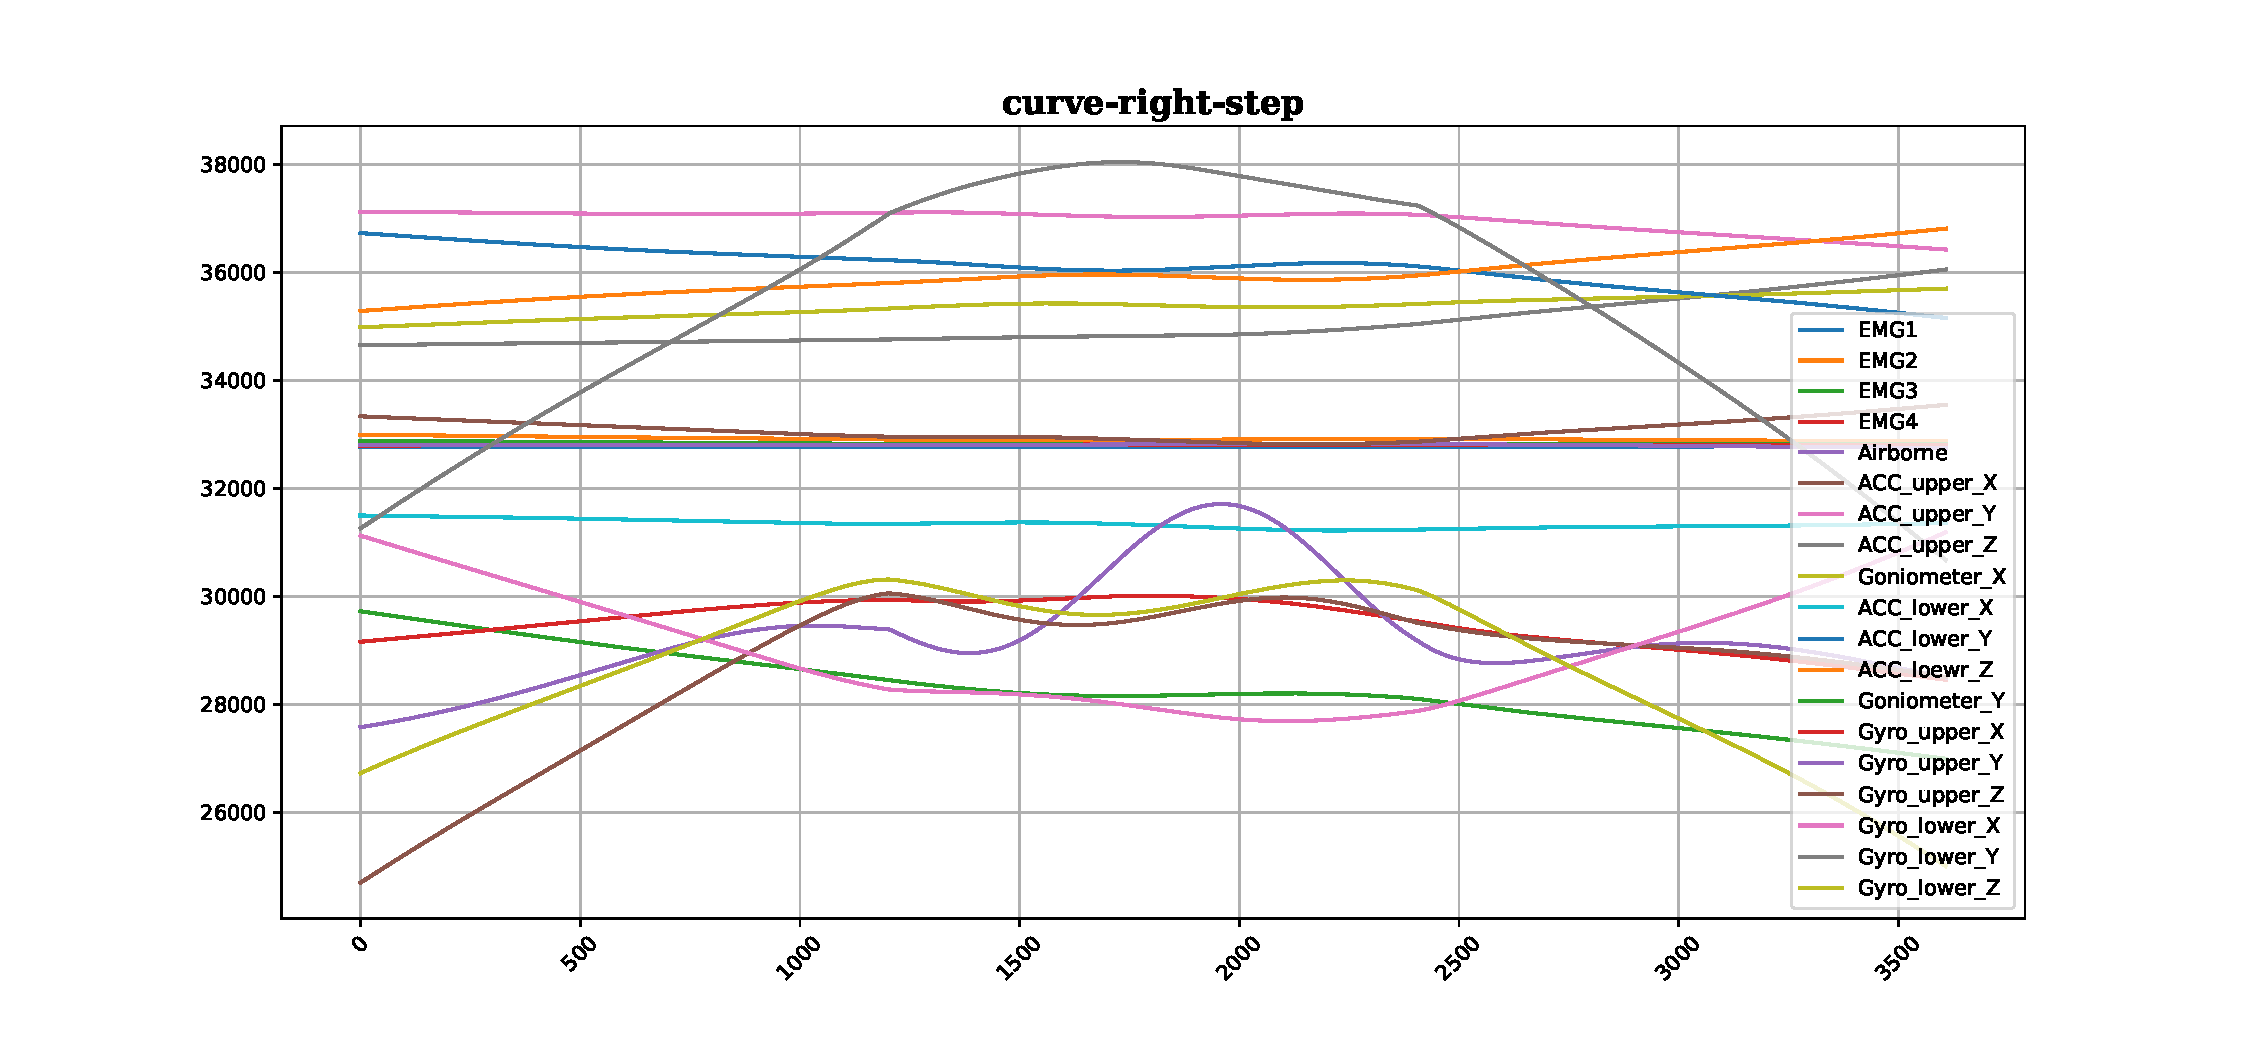
\includegraphics[width=\textwidth]{images/curve-right-step_example.pdf}
		\caption{curRight-step}
	\end{minipage}
\end{figure}



\begin{figure}[!tbp]
	\begin{minipage}[b]{0.31\textwidth}
		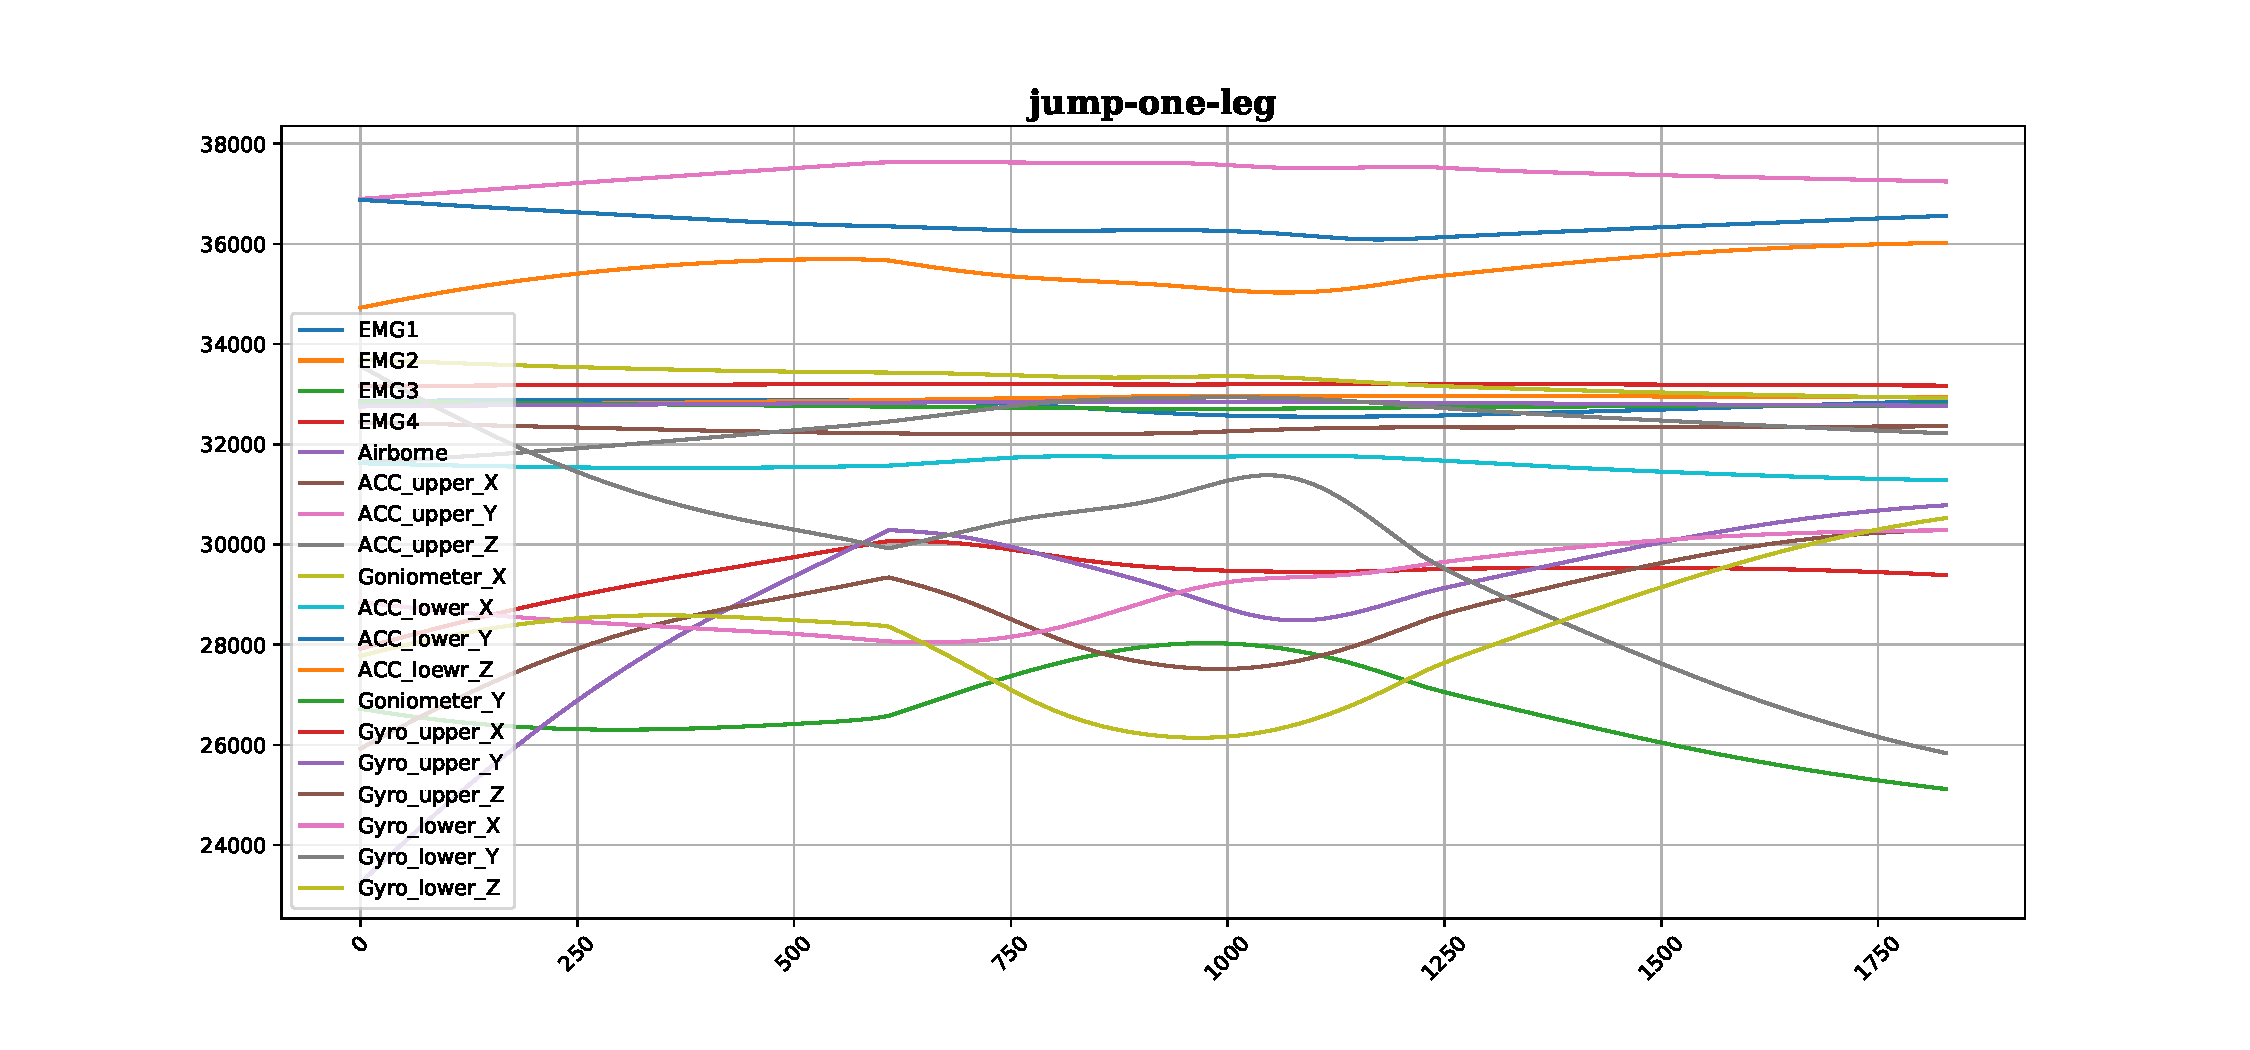
\includegraphics[width=\textwidth]{images/jump-one-leg_example.pdf}
		\caption{jump-one-leg}
	\end{minipage}
	\begin{minipage}[b]{0.31\textwidth}
		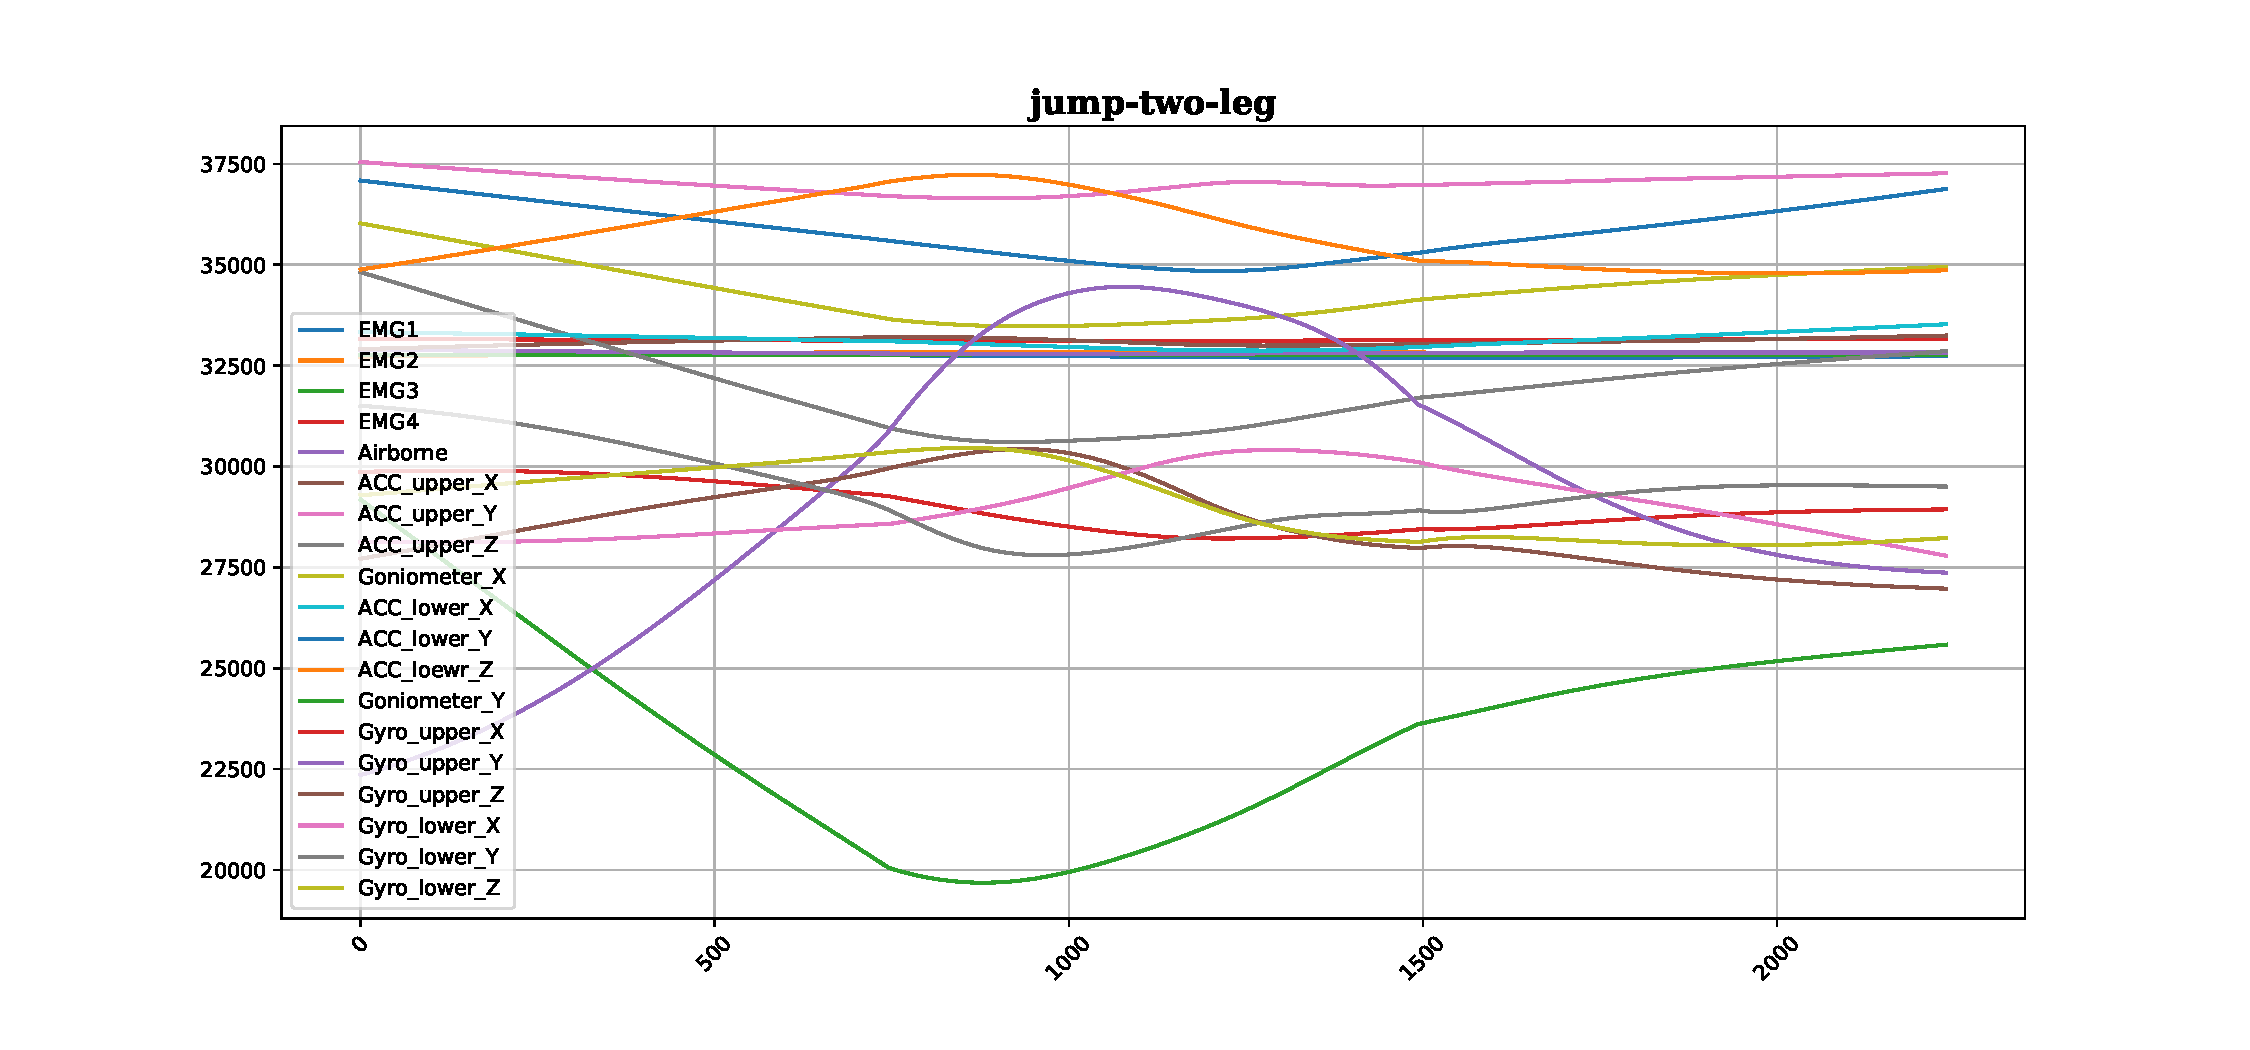
\includegraphics[width=\textwidth]{images/jump-two-leg_example.pdf}
		\caption{jump-two-leg}
	\end{minipage}
	\begin{minipage}[b]{0.31\textwidth}
		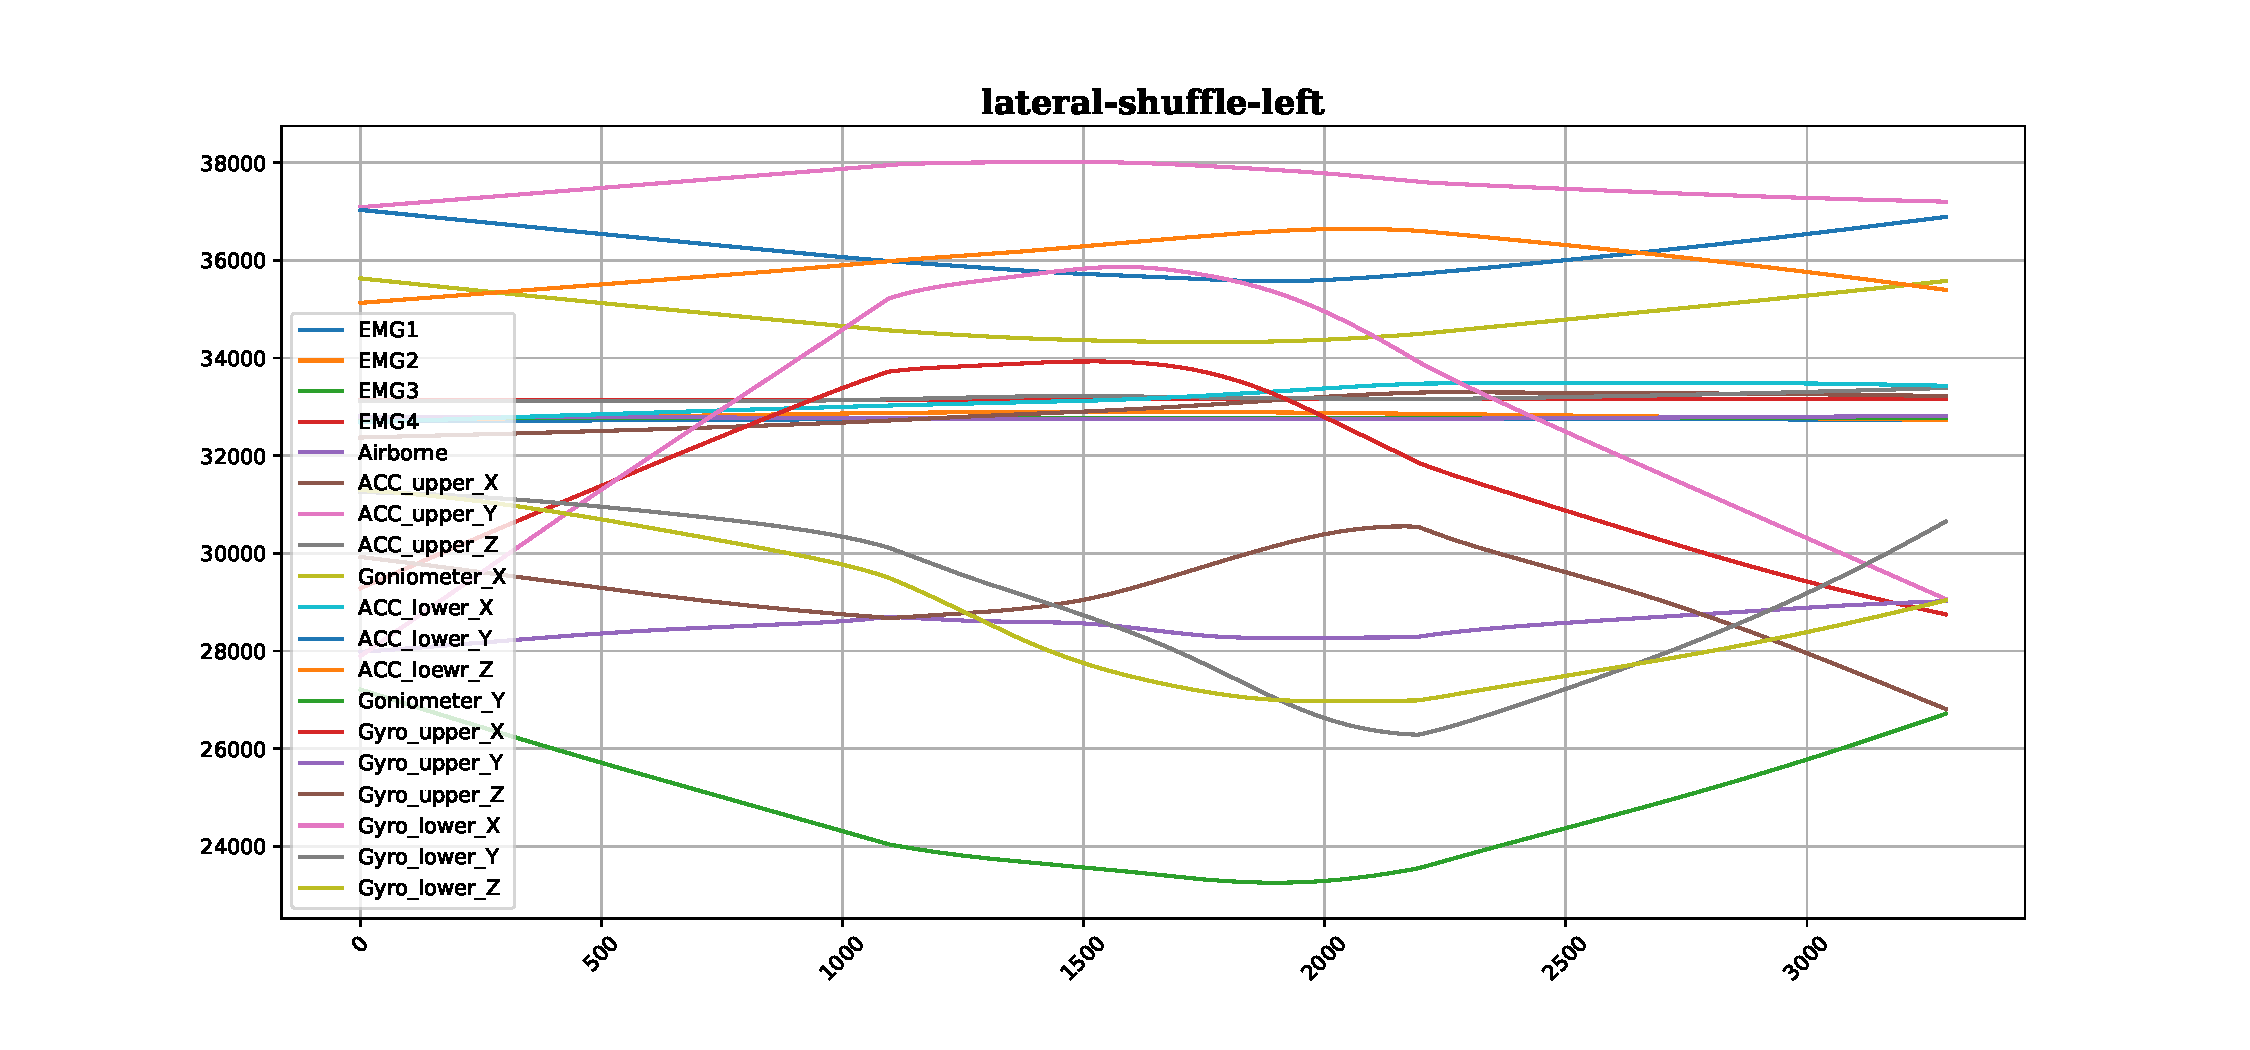
\includegraphics[width=\textwidth]{images/lateral-shuffle-left_example.pdf}
		\caption{lateral-shuffle-left}
	\end{minipage}
\end{figure}


\begin{figure}[!tbp]
	\begin{minipage}[b]{0.31\textwidth}
		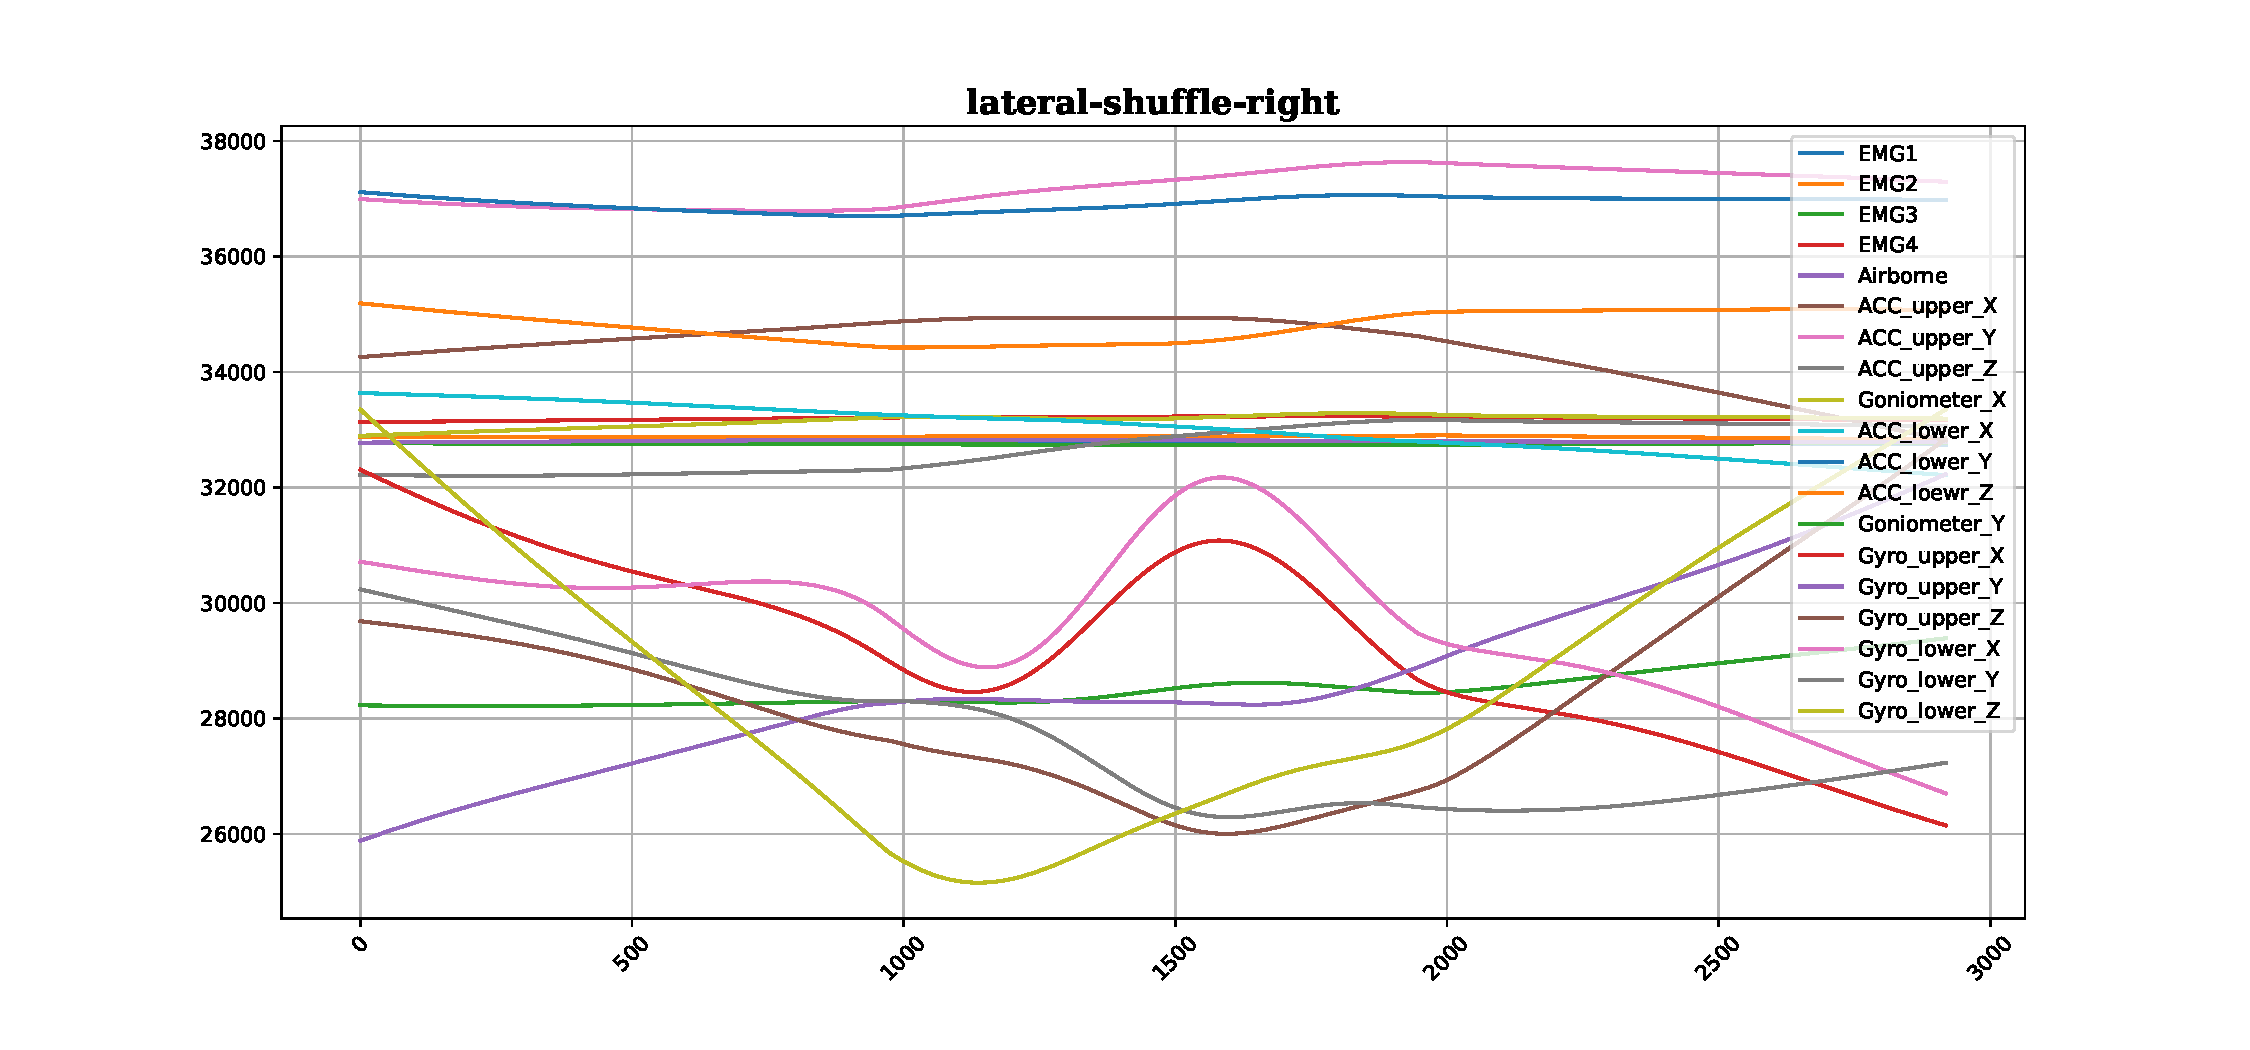
\includegraphics[width=\textwidth]{images/lateral-shuffle-right_example.pdf}
		\caption{lateral-shuffle-right}
	\end{minipage}
	\begin{minipage}[b]{0.31\textwidth}
		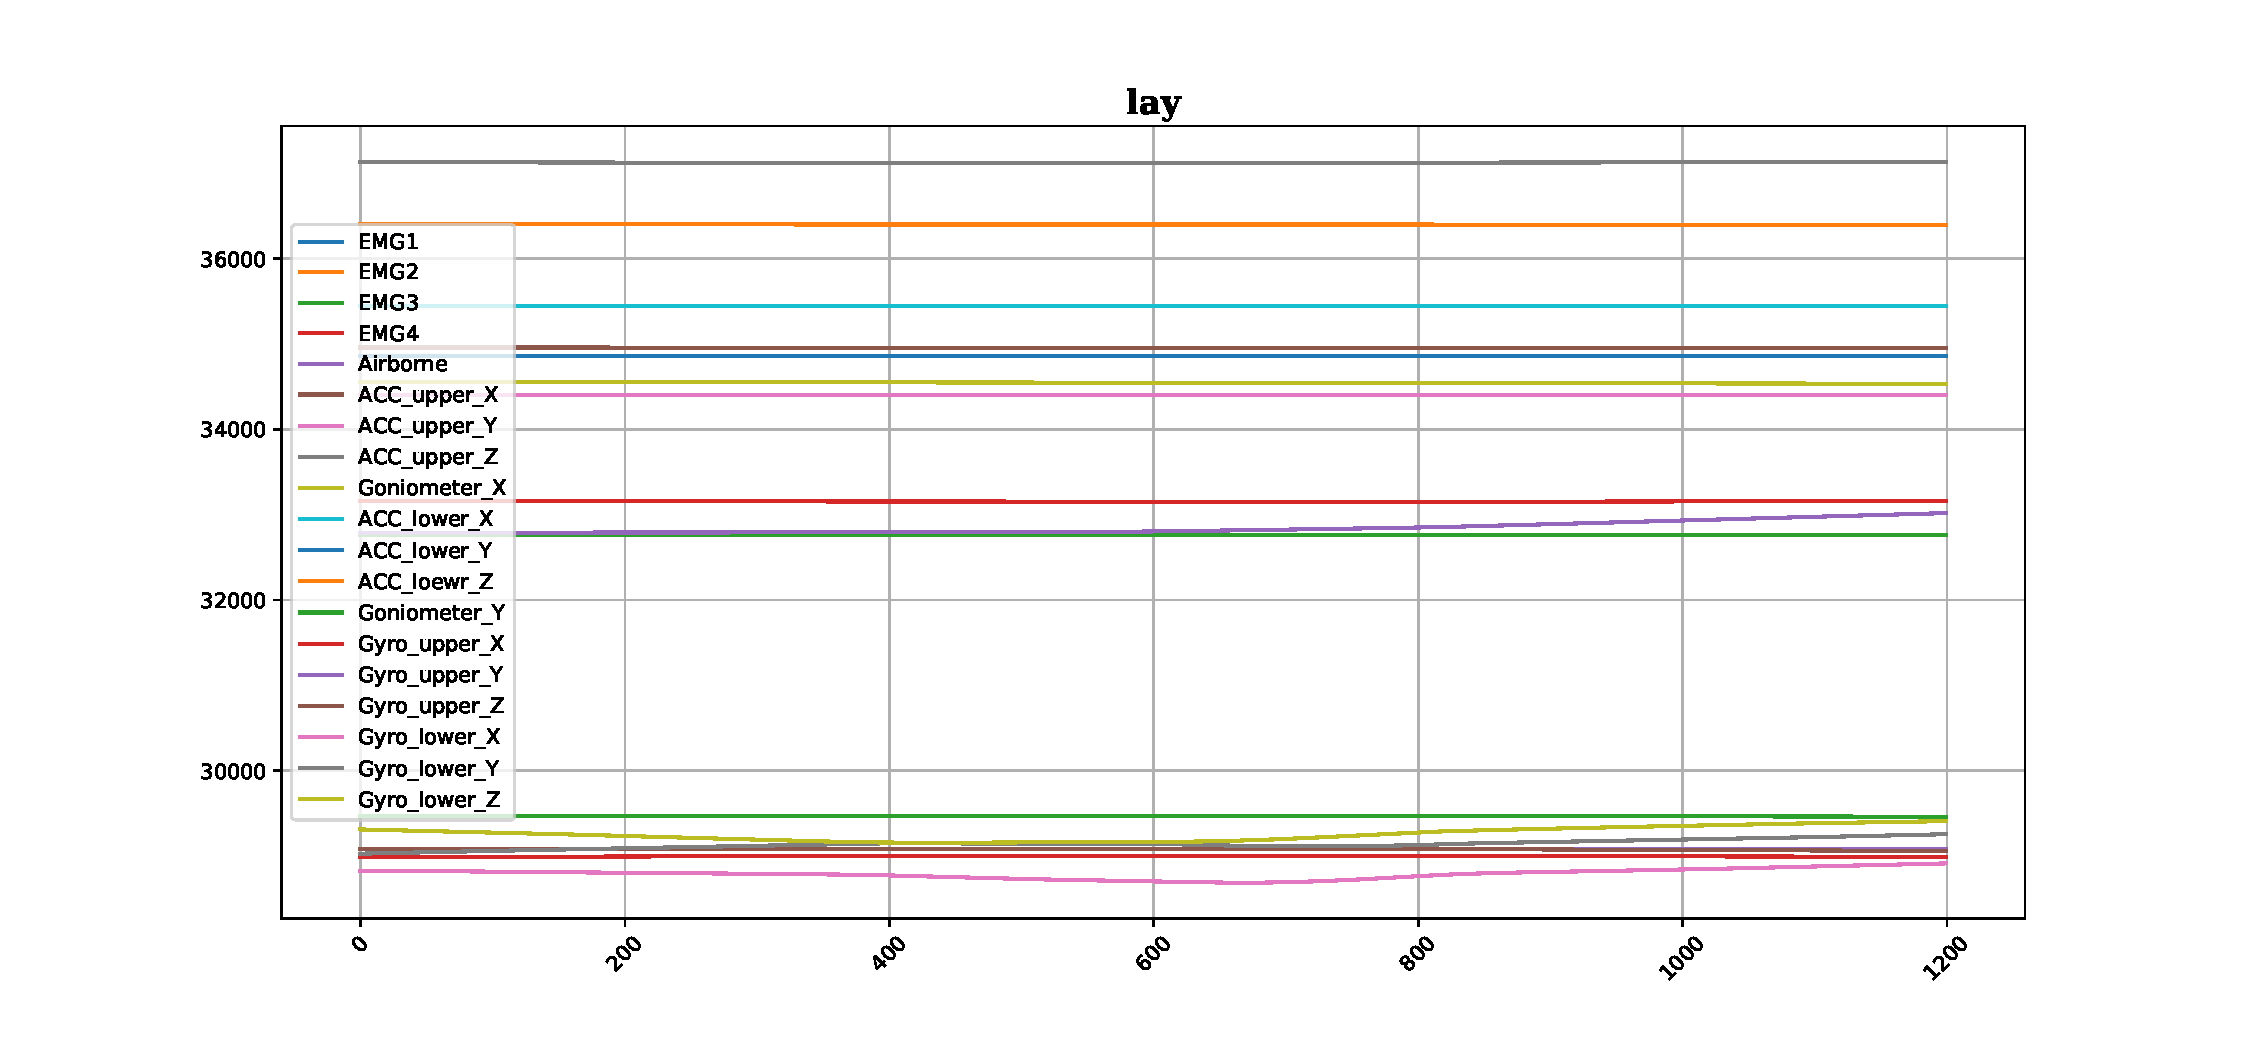
\includegraphics[width=\textwidth]{images/lay_example.pdf}
		\caption{lay}
	\end{minipage}
	\begin{minipage}[b]{0.31\textwidth}
		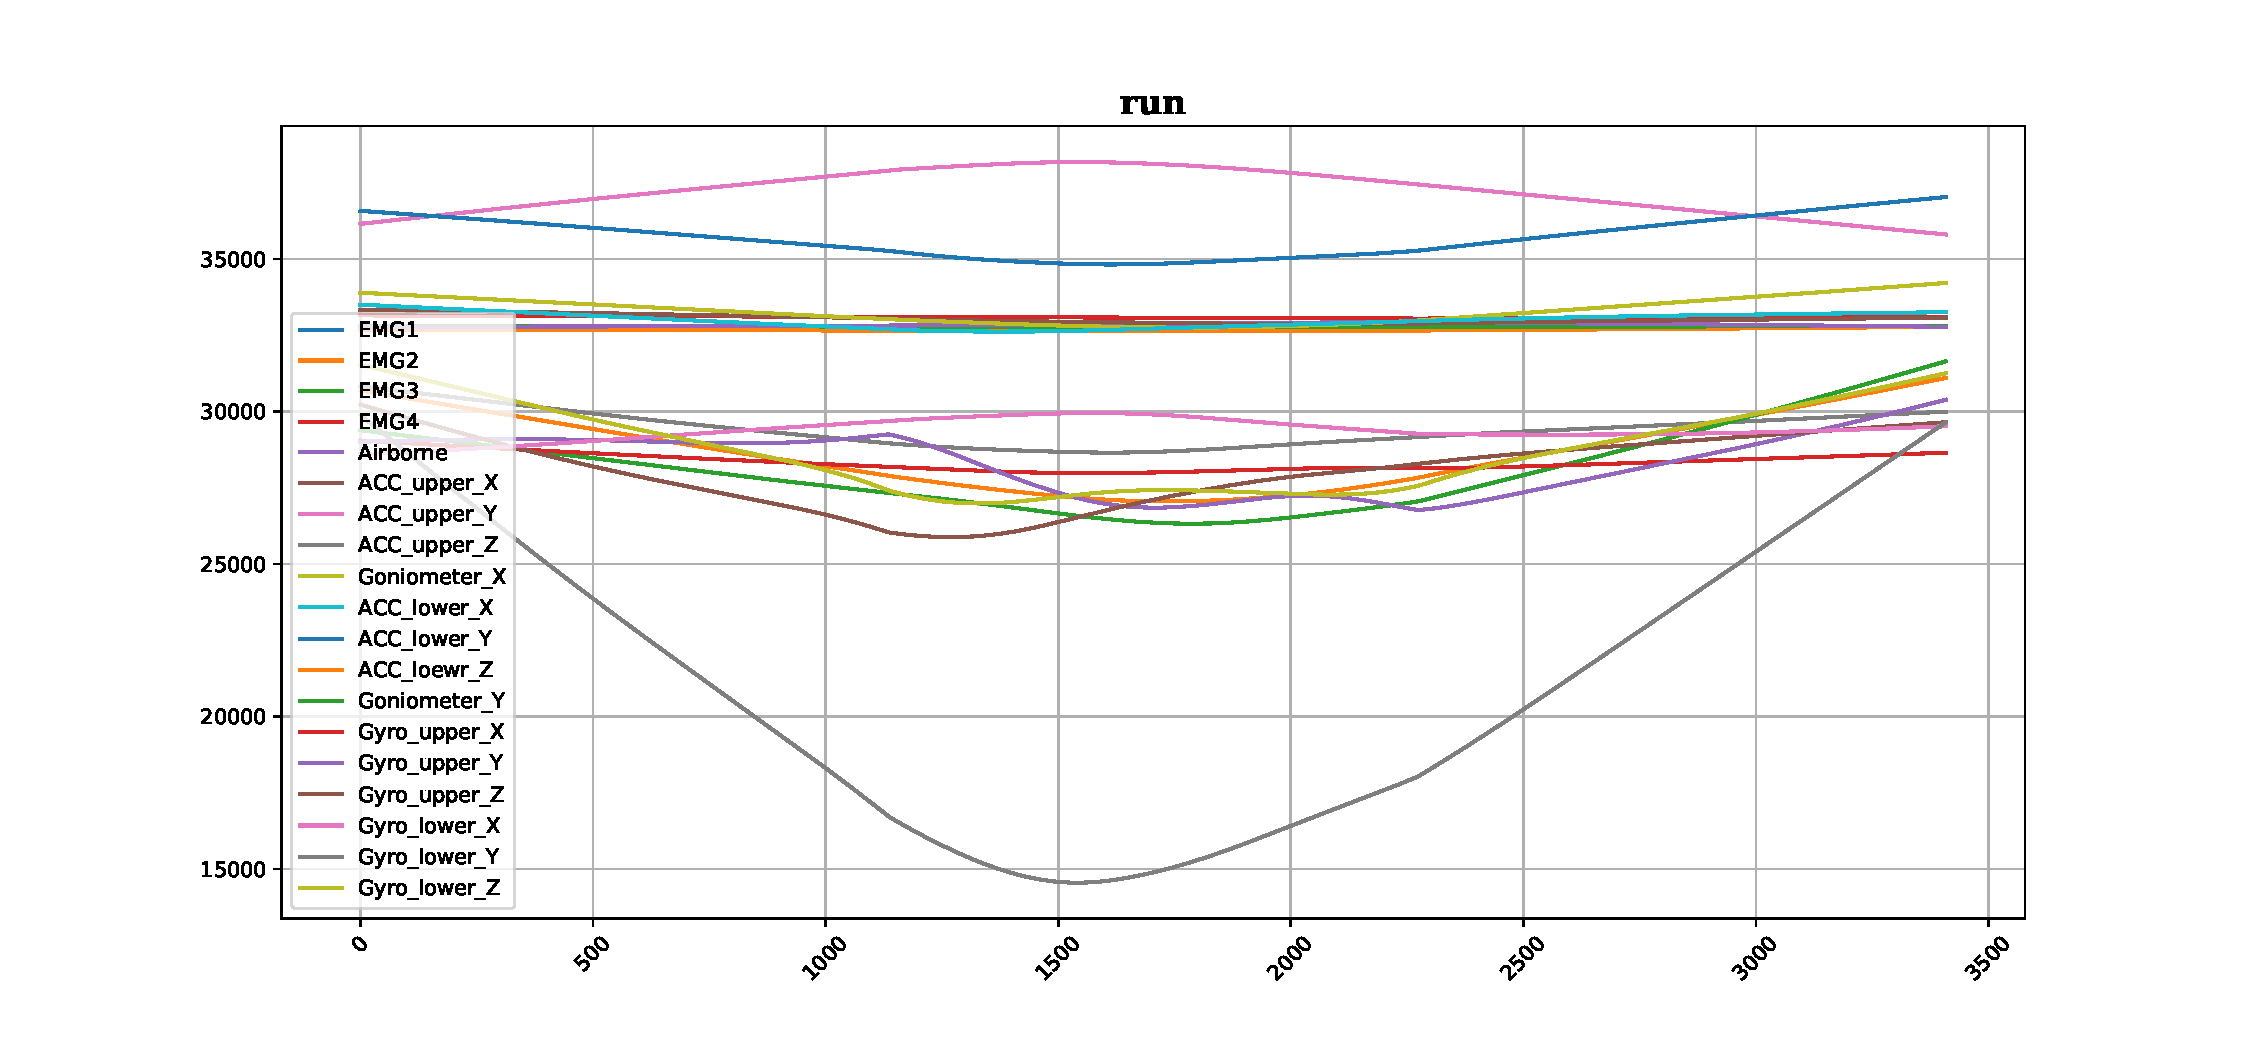
\includegraphics[width=\textwidth]{images/run_example.pdf}
		\caption{run}
	\end{minipage}
\end{figure}



\begin{figure}[!tbp]
	\begin{minipage}[b]{0.31\textwidth}
		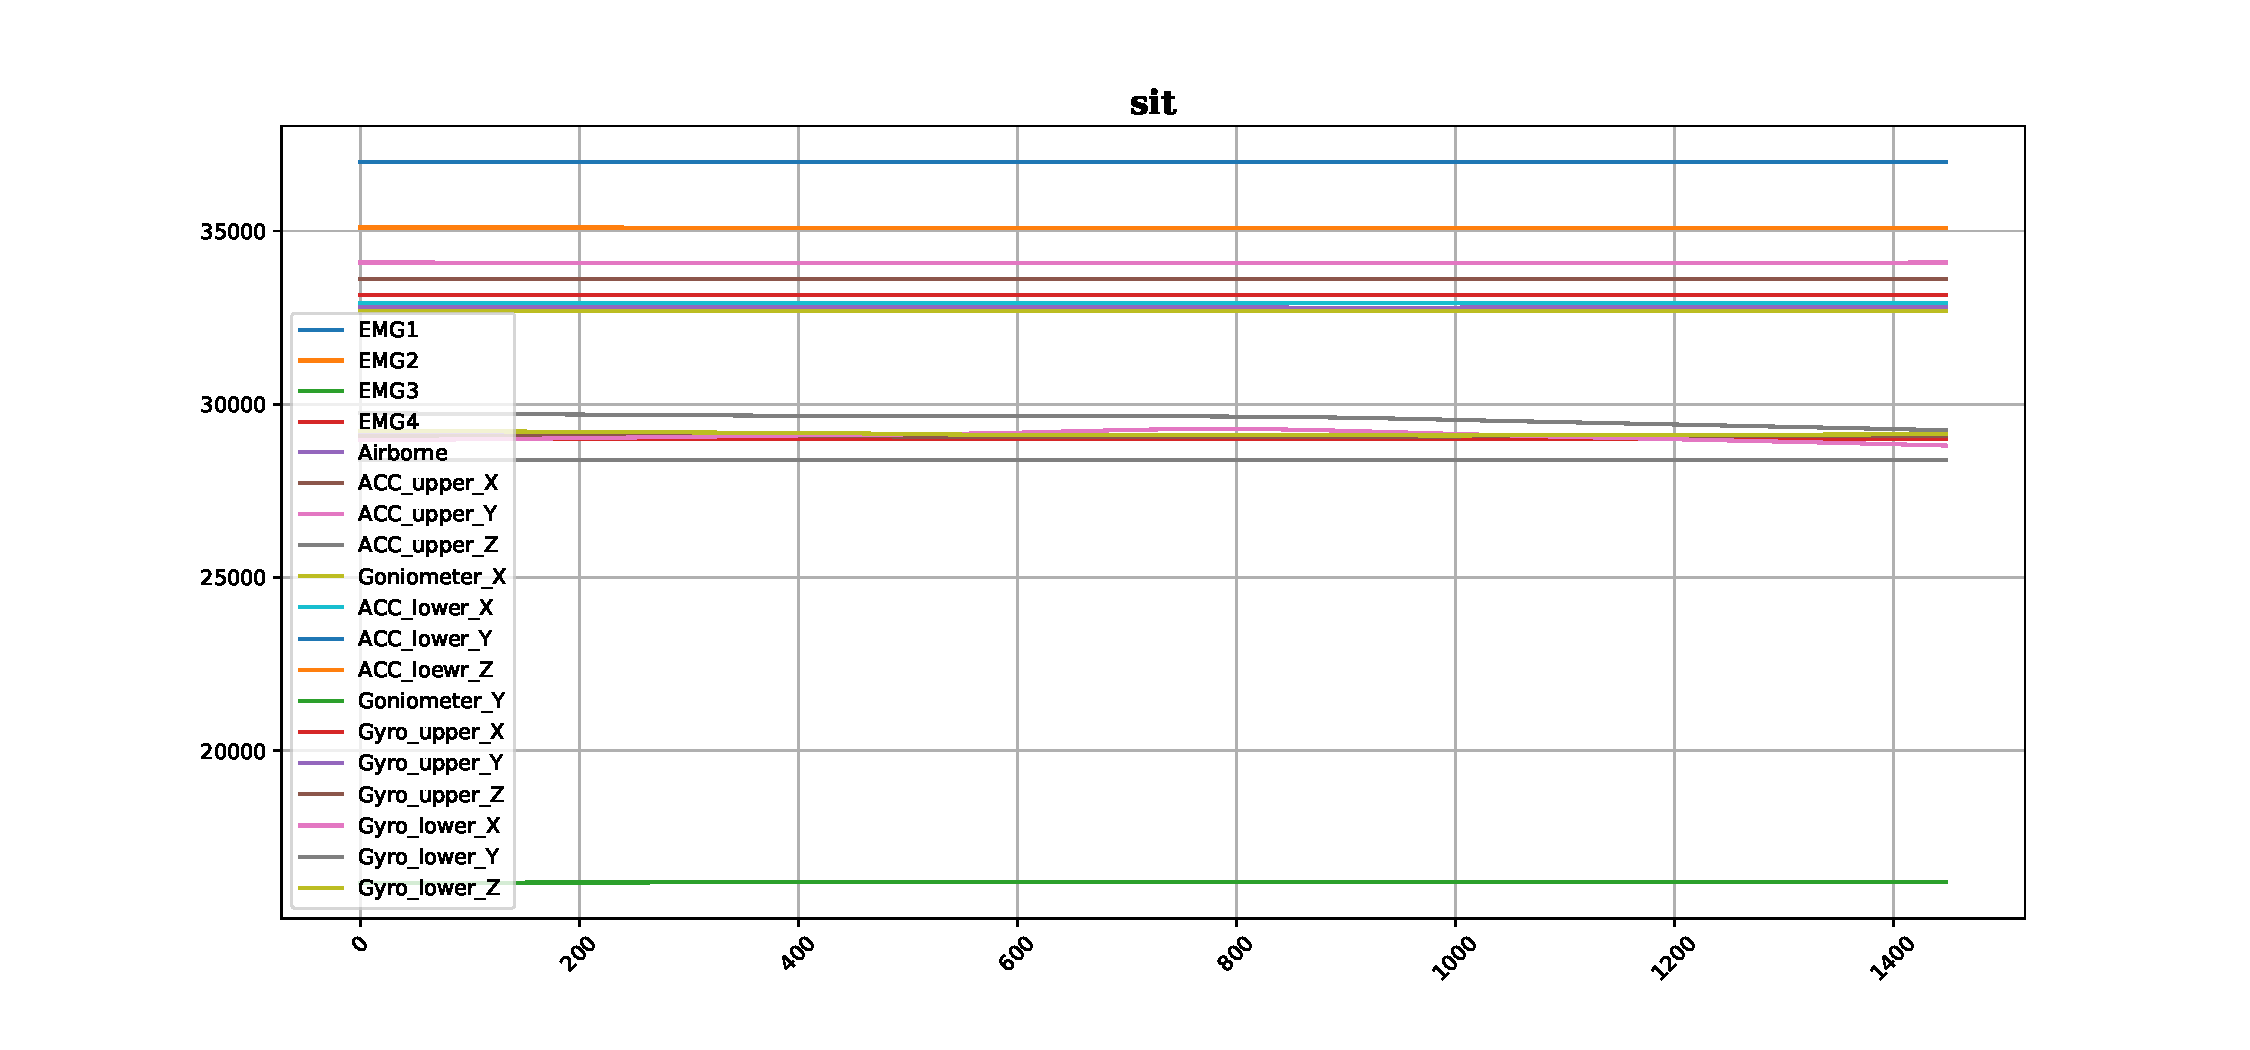
\includegraphics[width=\textwidth]{images/sit_example.pdf}
		\caption{sit}
	\end{minipage}
	\begin{minipage}[b]{0.31\textwidth}
		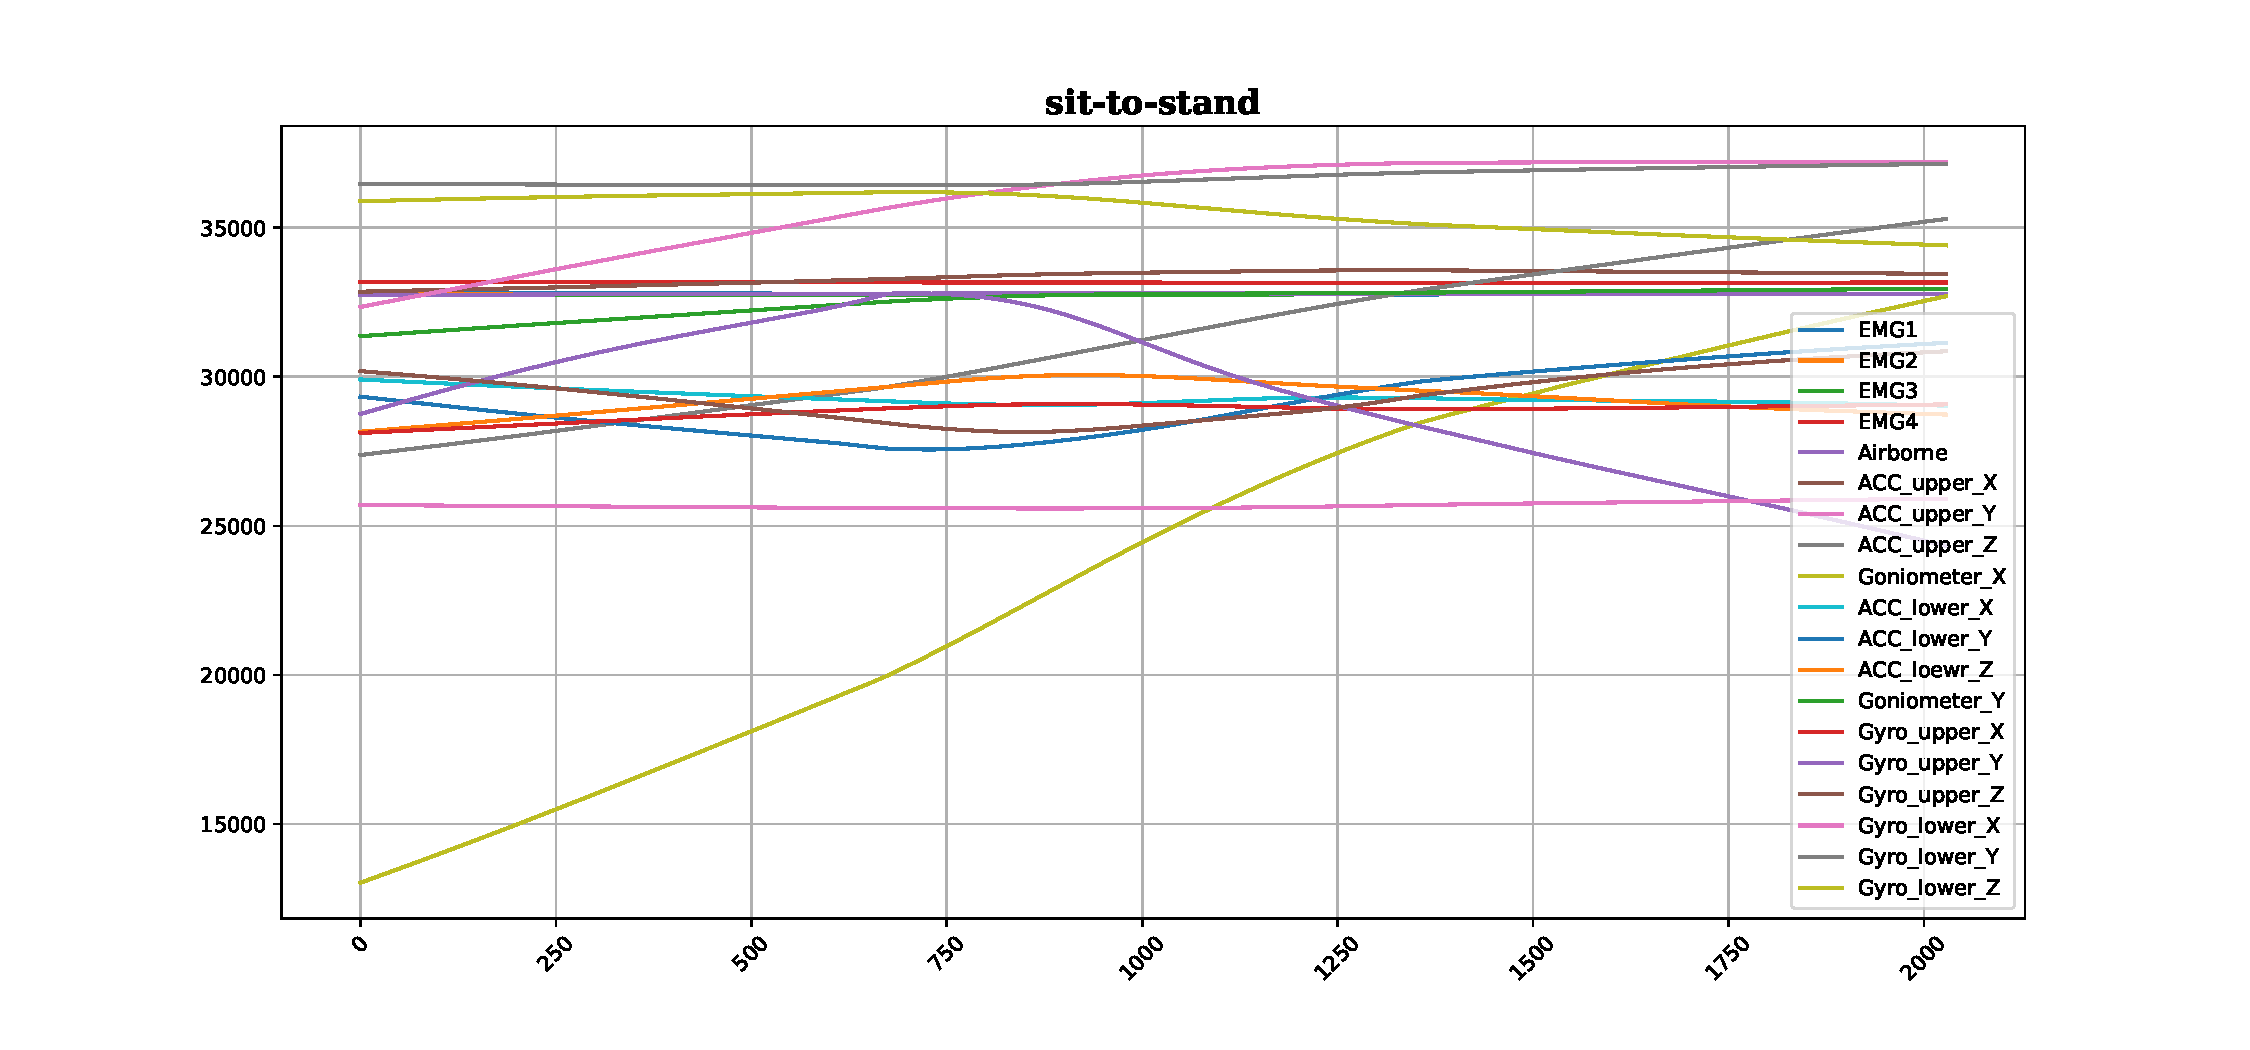
\includegraphics[width=\textwidth]{images/sit-to-stand_example.pdf}
		\caption{sit-to-stand}
	\end{minipage}
	\begin{minipage}[b]{0.31\textwidth}
		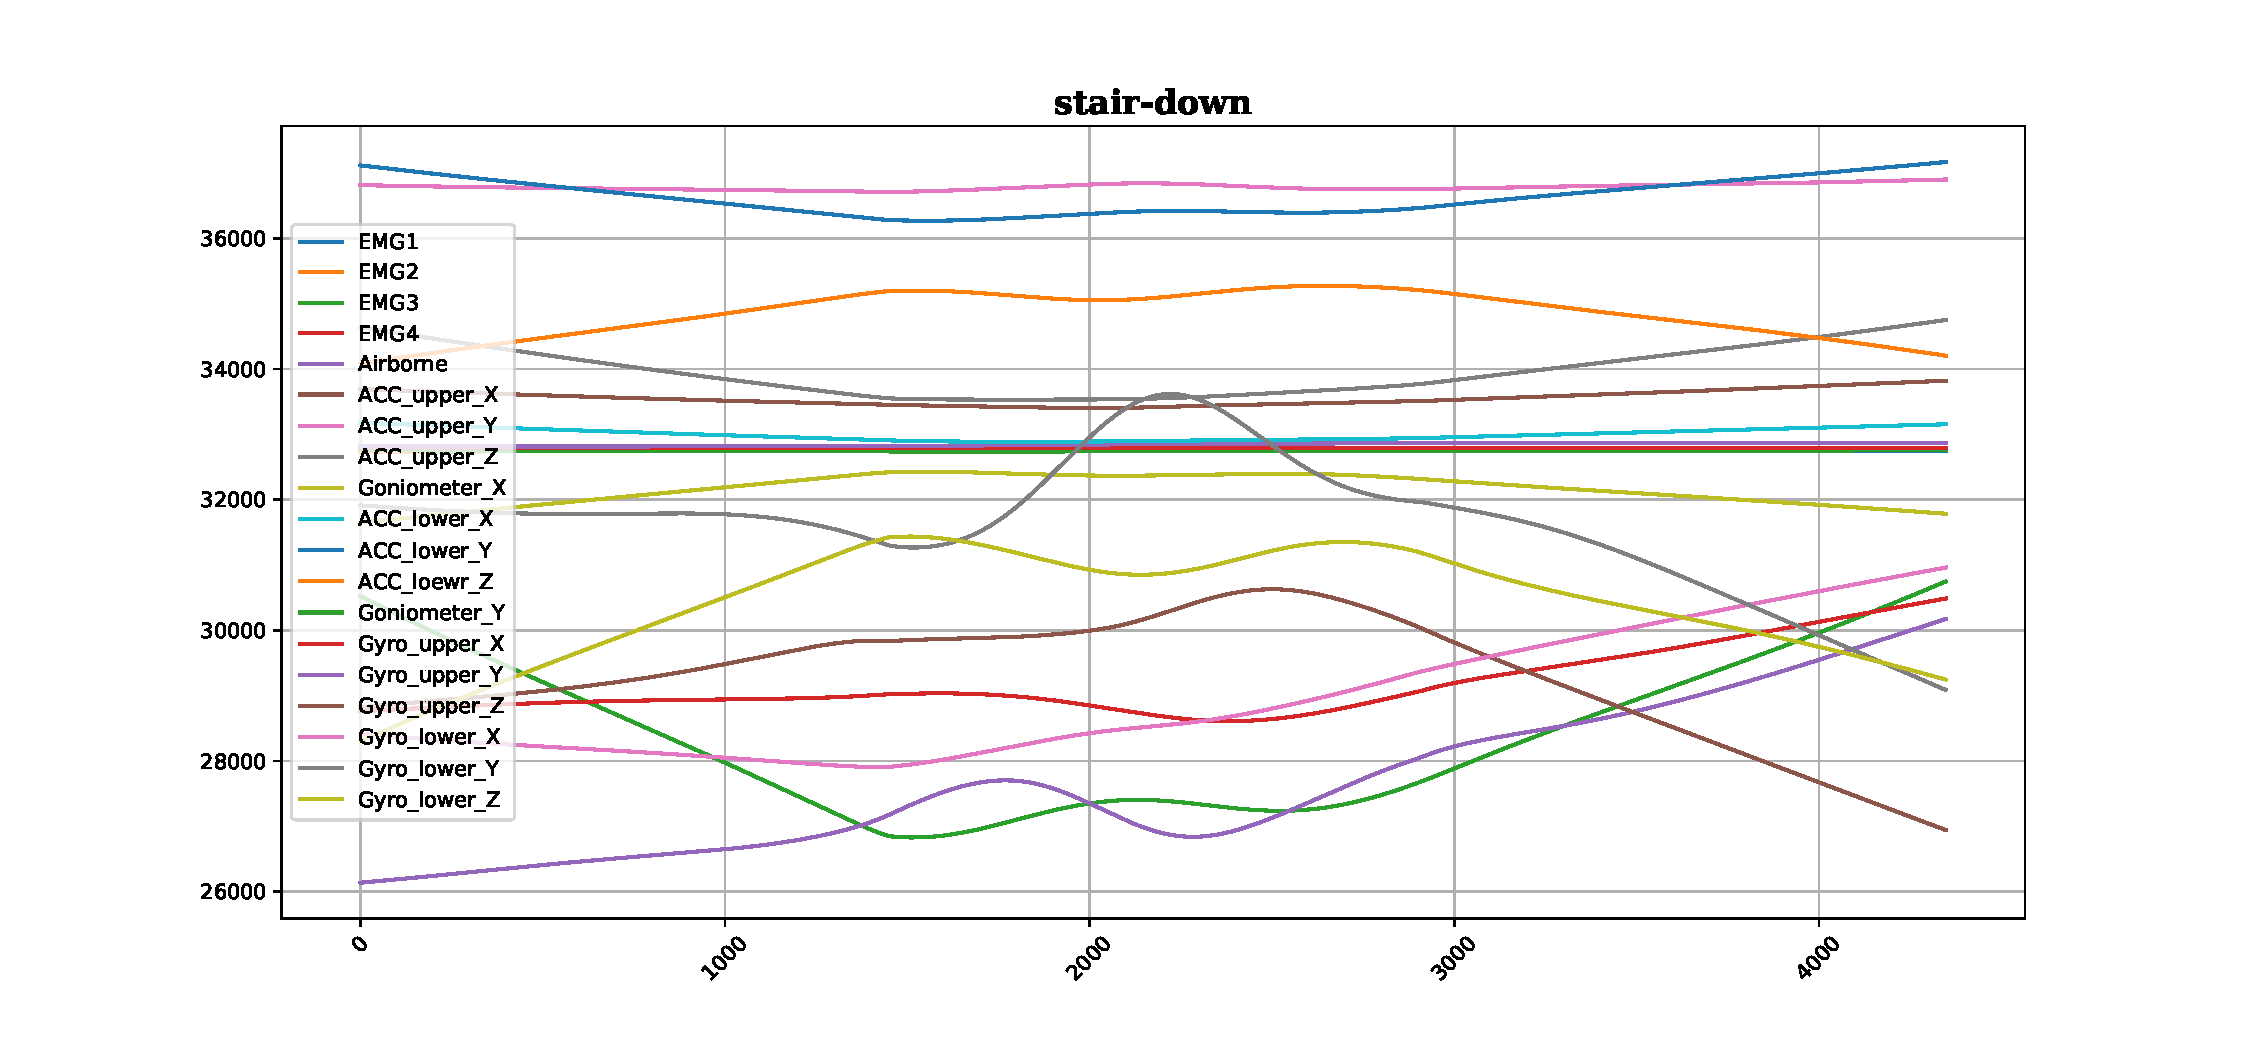
\includegraphics[width=\textwidth]{images/stair-down_example.pdf}
		\caption{stair-down}
	\end{minipage}
\end{figure}


\begin{figure}[!tbp]
	\begin{minipage}[b]{0.31\textwidth}
		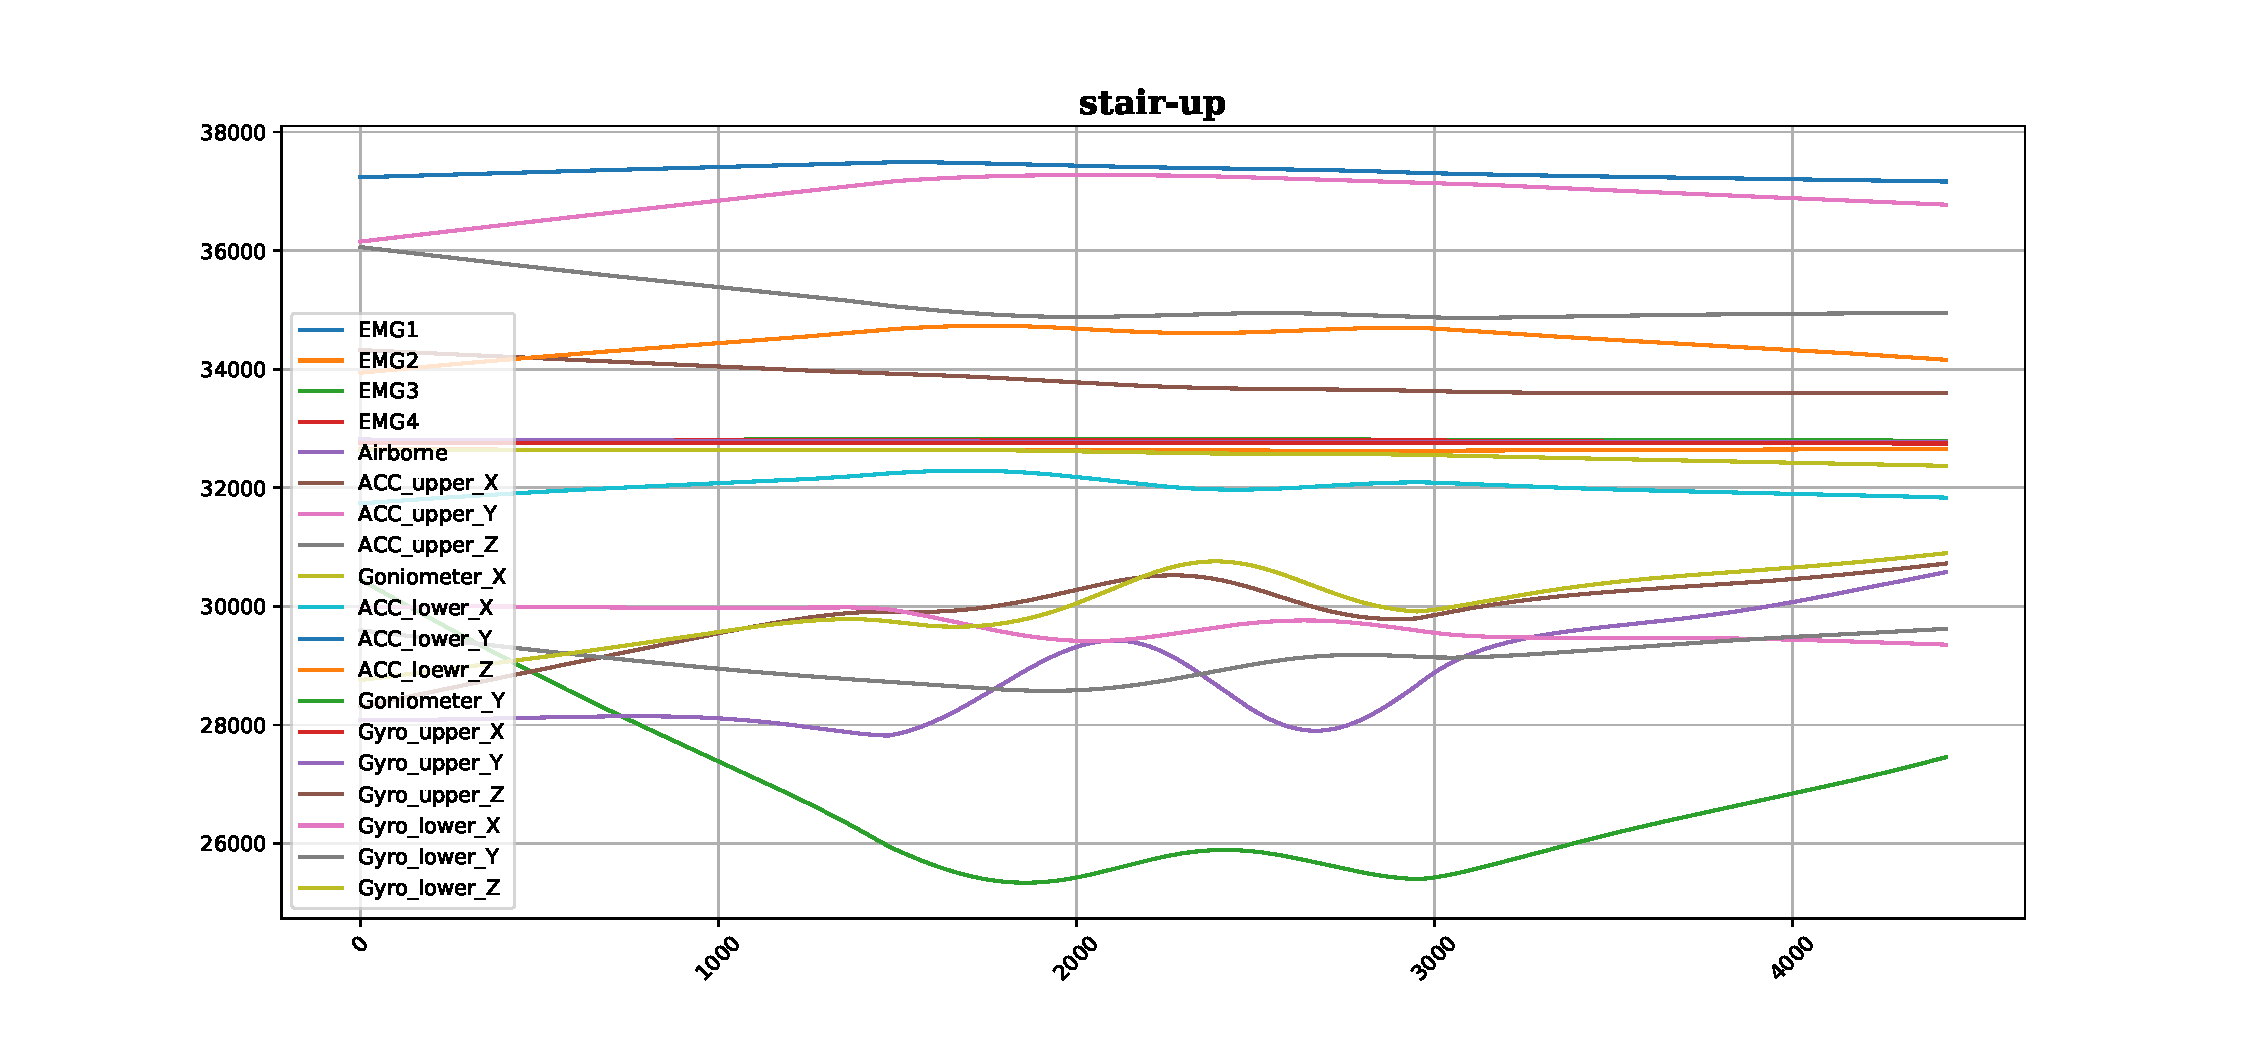
\includegraphics[width=\textwidth]{images/stair-up_example.pdf}
		\caption{stair-up}
	\end{minipage}
	\begin{minipage}[b]{0.31\textwidth}
		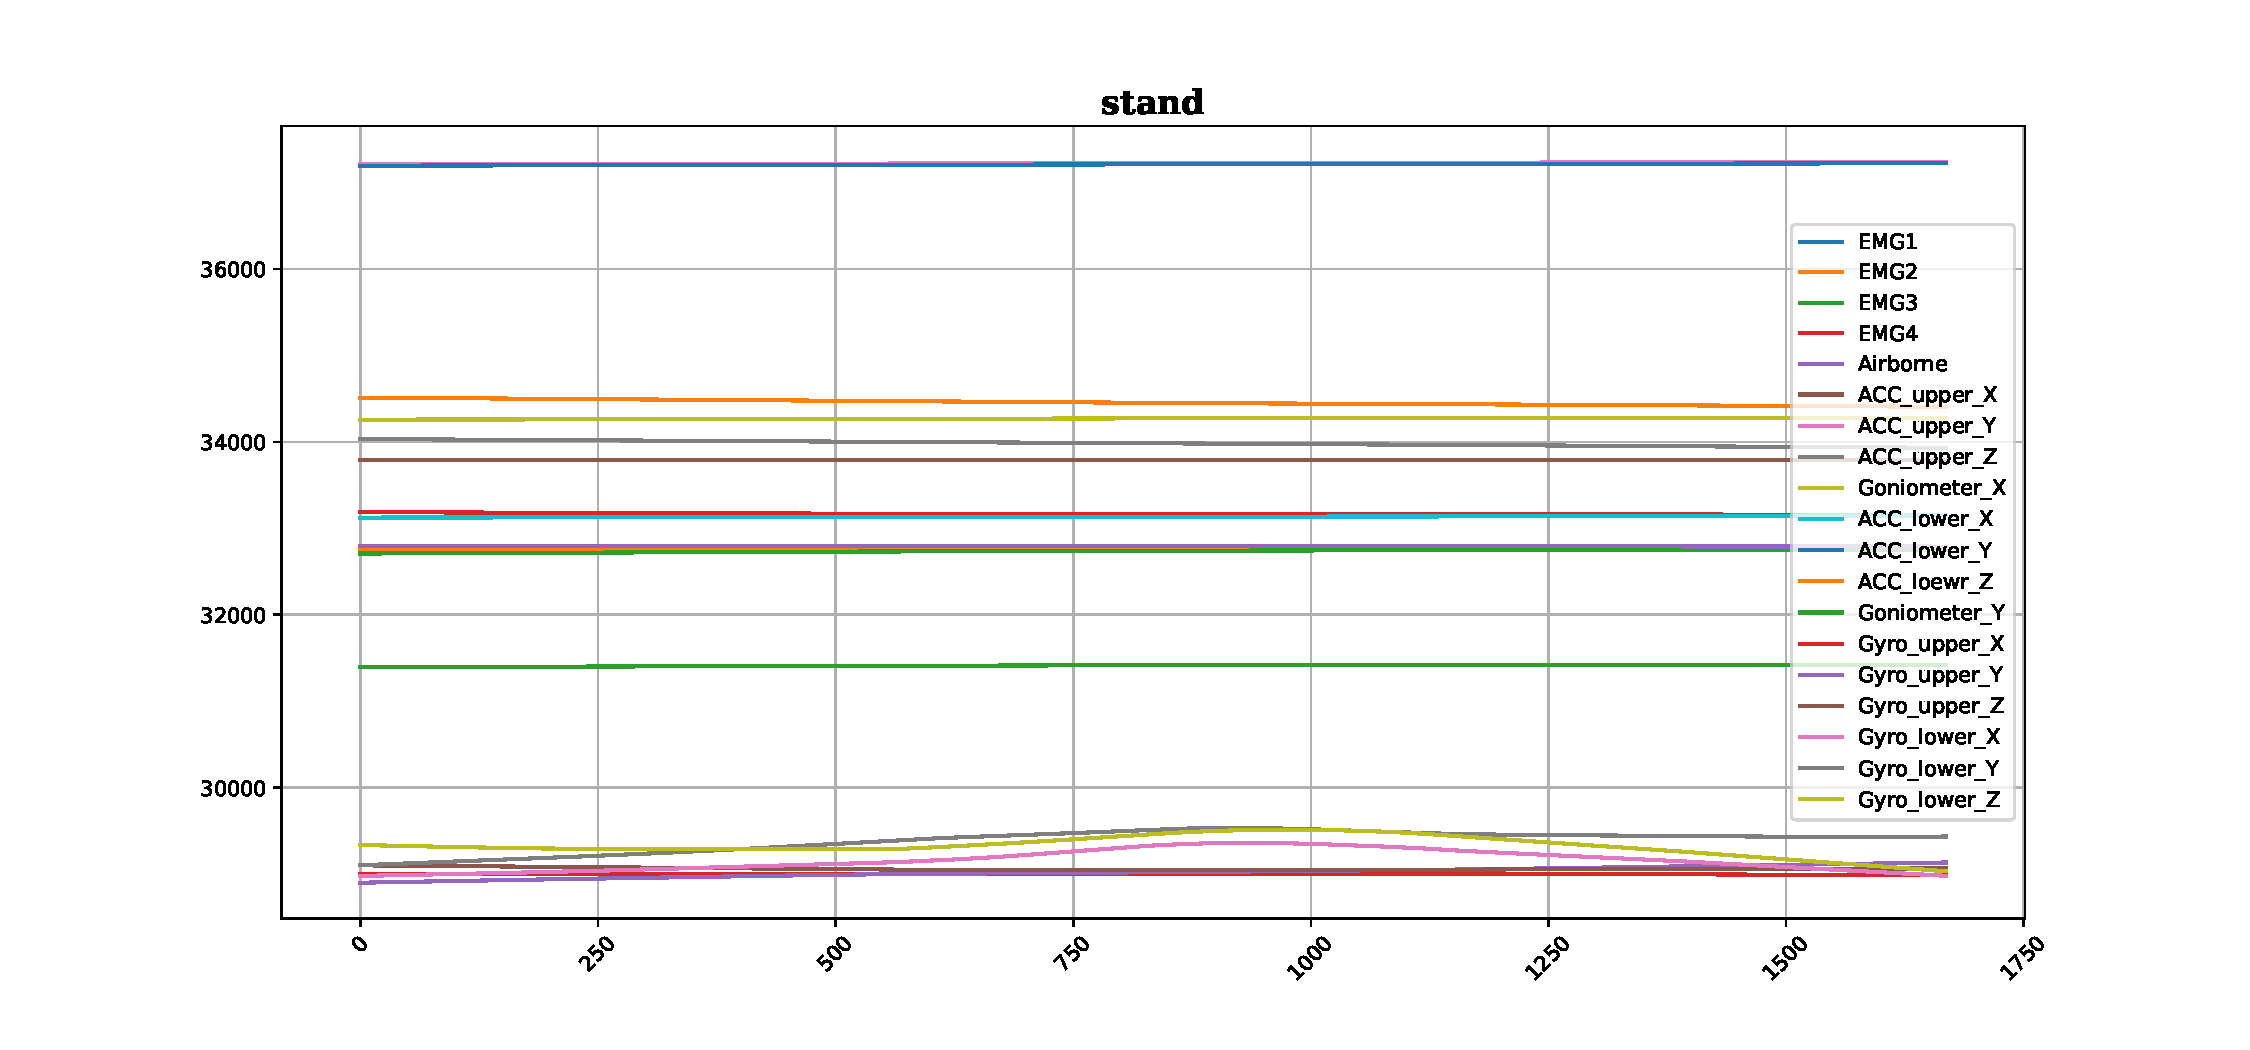
\includegraphics[width=\textwidth]{images/stand_example.pdf}
		\caption{stand}
	\end{minipage}
	\begin{minipage}[b]{0.31\textwidth}
		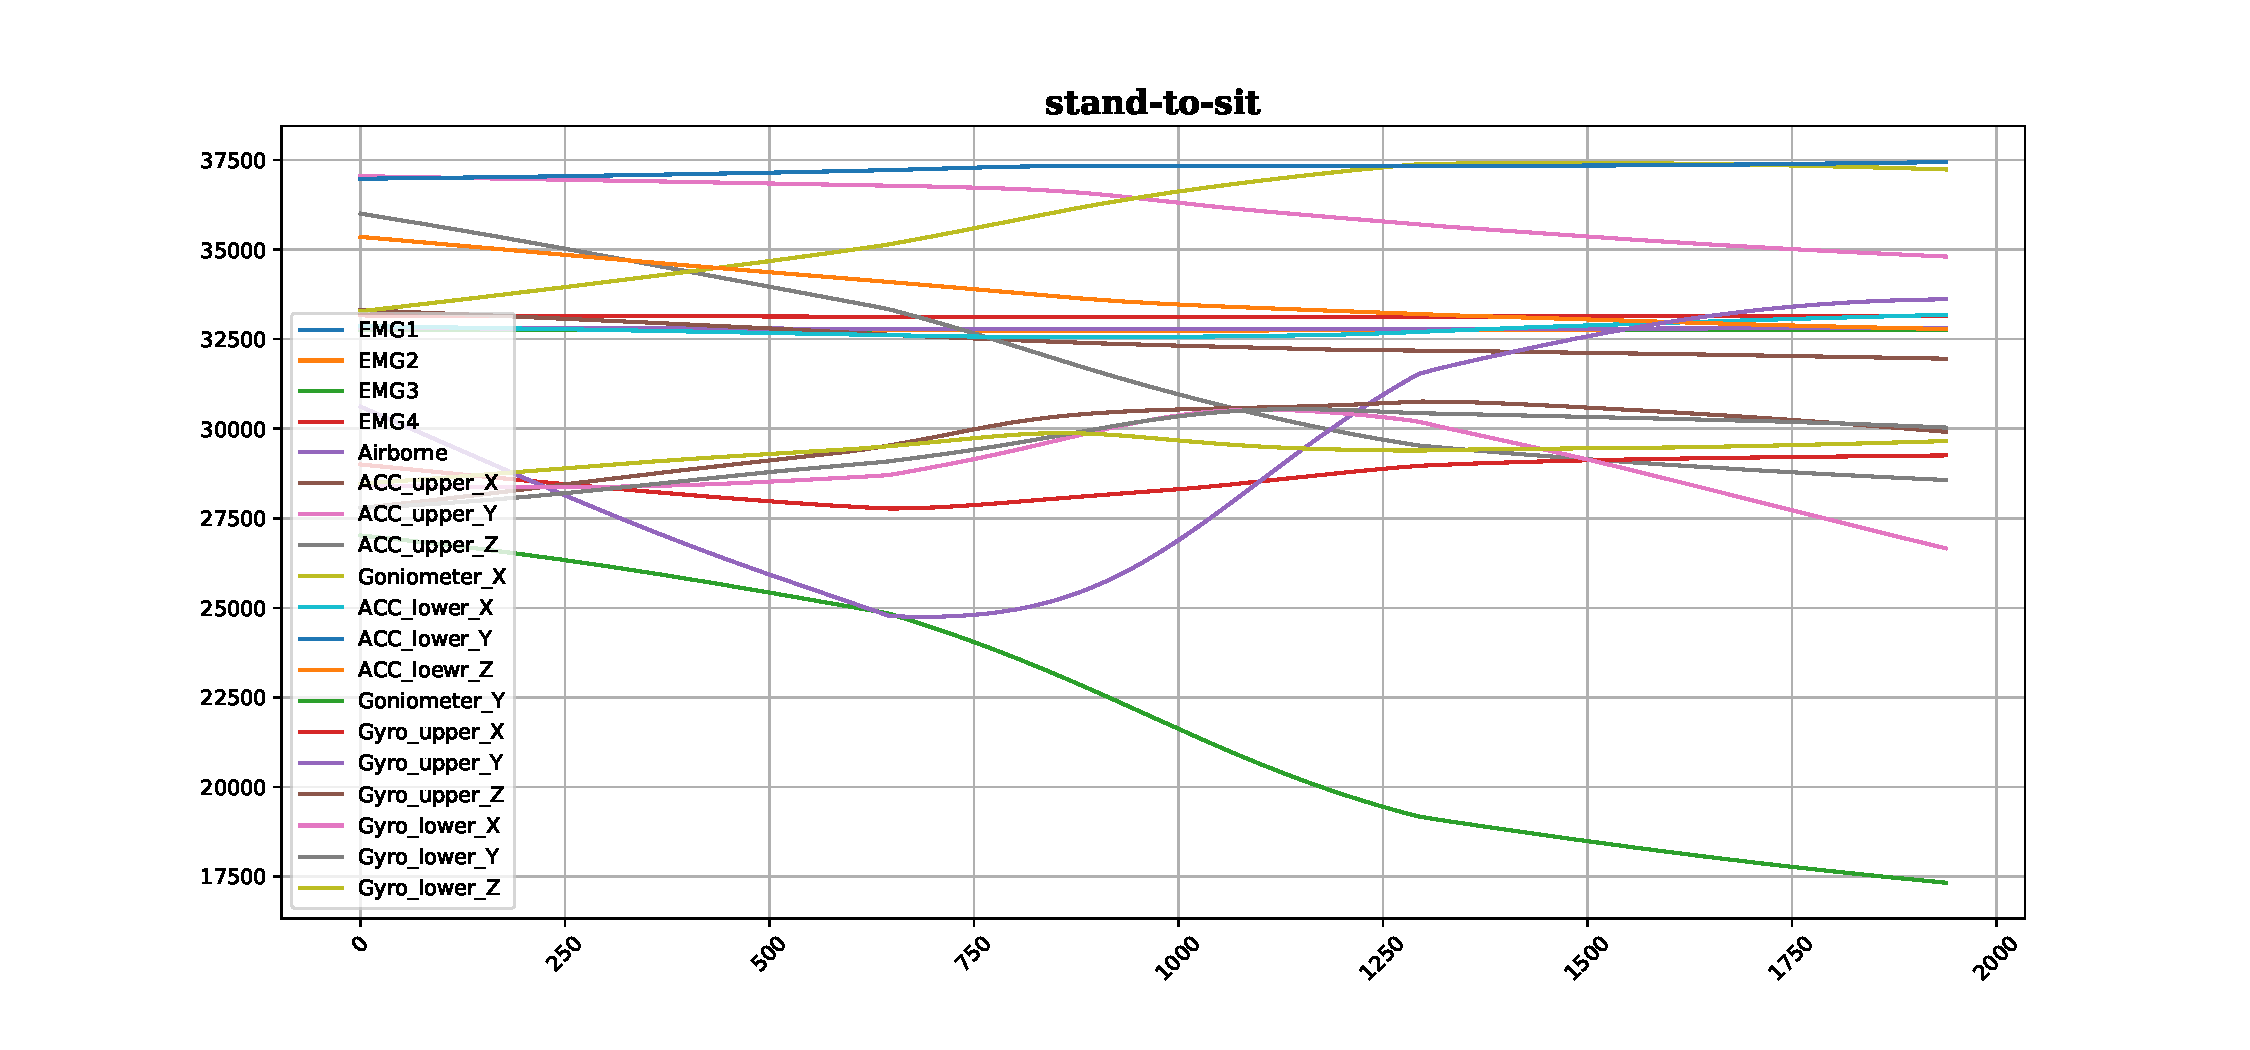
\includegraphics[width=\textwidth]{images/stand-to-sit_example.pdf}
		\caption{stand-to-sit}
	\end{minipage}
\end{figure}

\begin{figure}[!tbp]
	\begin{minipage}[b]{0.31\textwidth}
		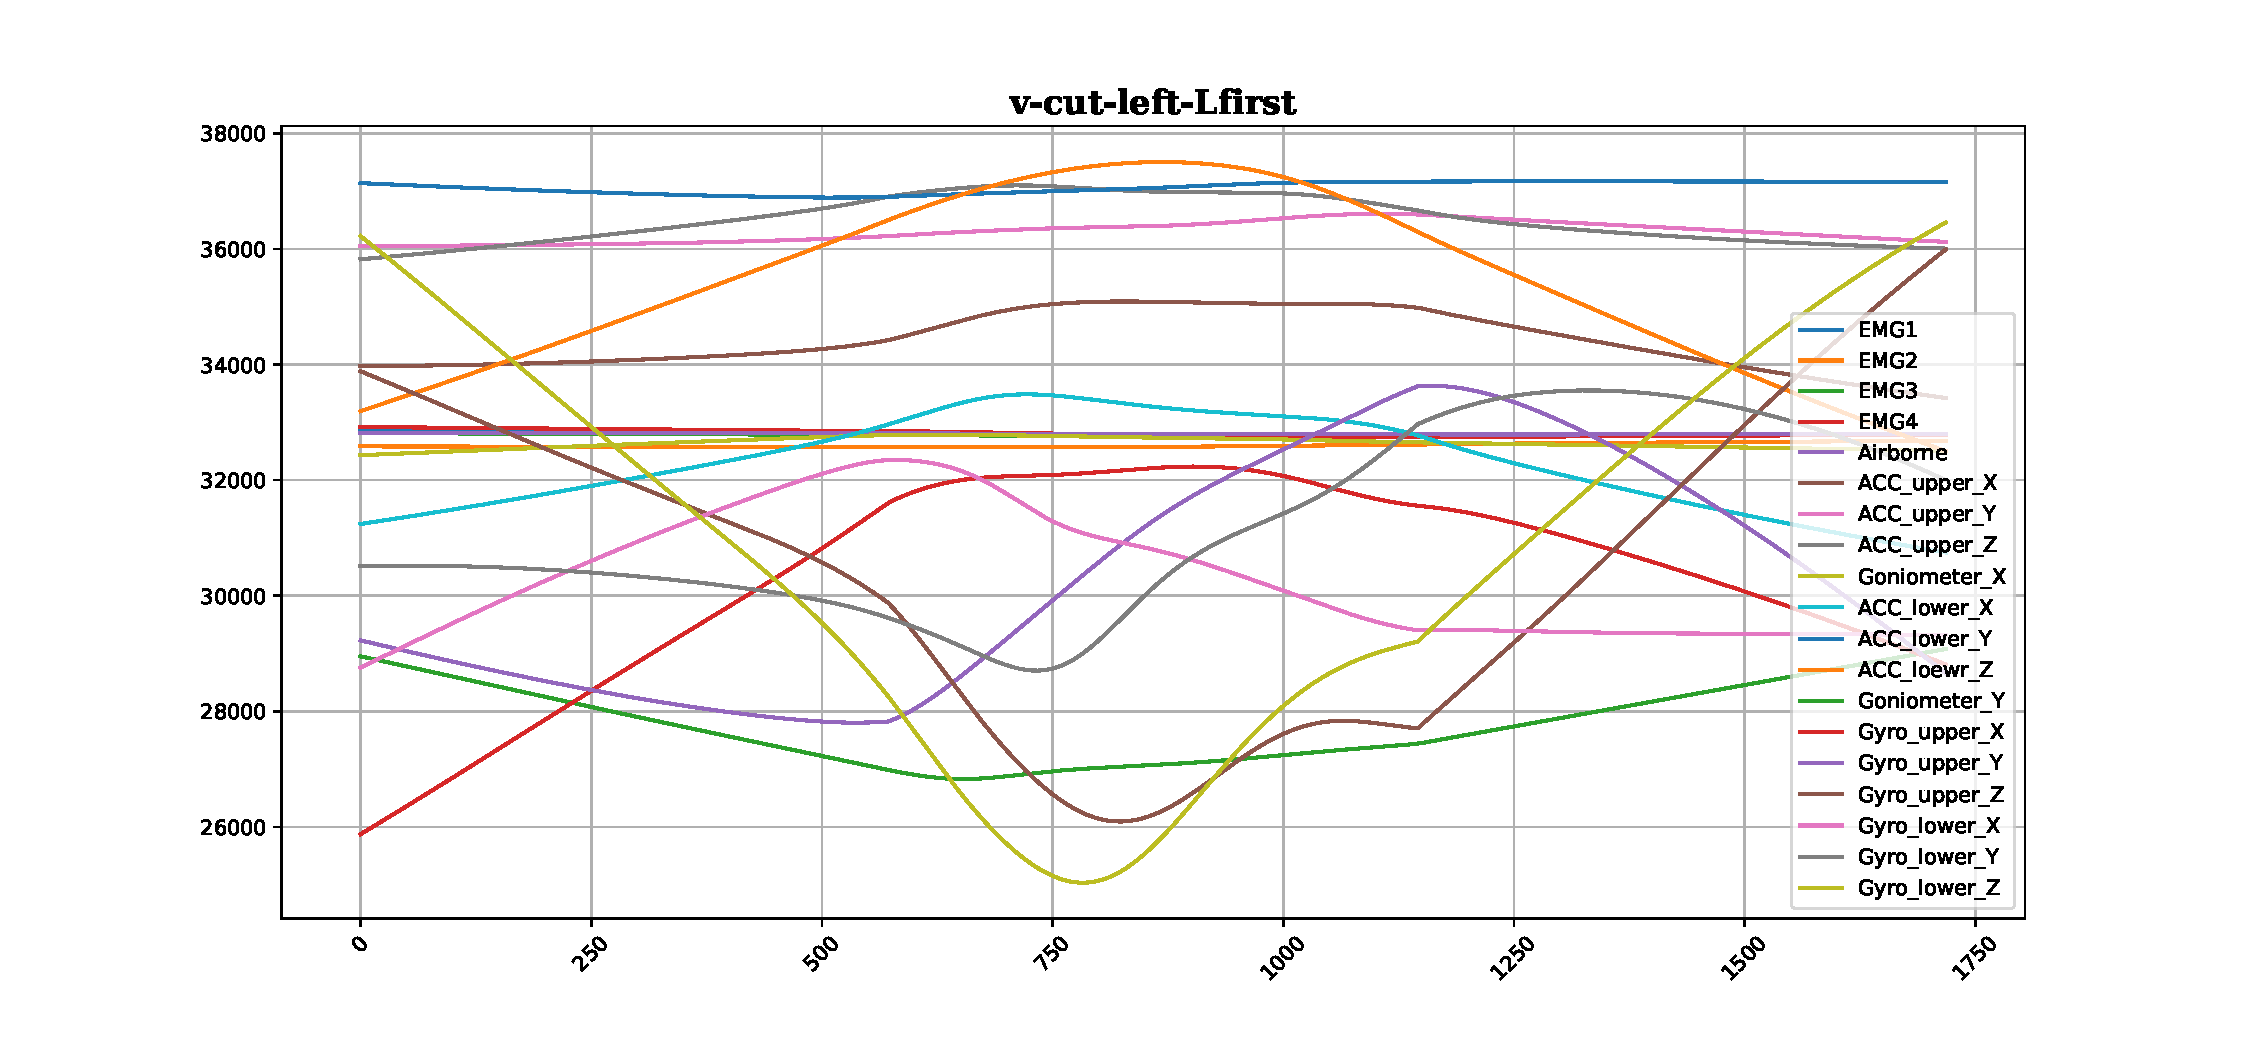
\includegraphics[width=\textwidth]{images/v-cut-left-Lfirst_example.pdf}
		\caption{v-cut-left-Lfirst}
	\end{minipage}
	\begin{minipage}[b]{0.31\textwidth}
		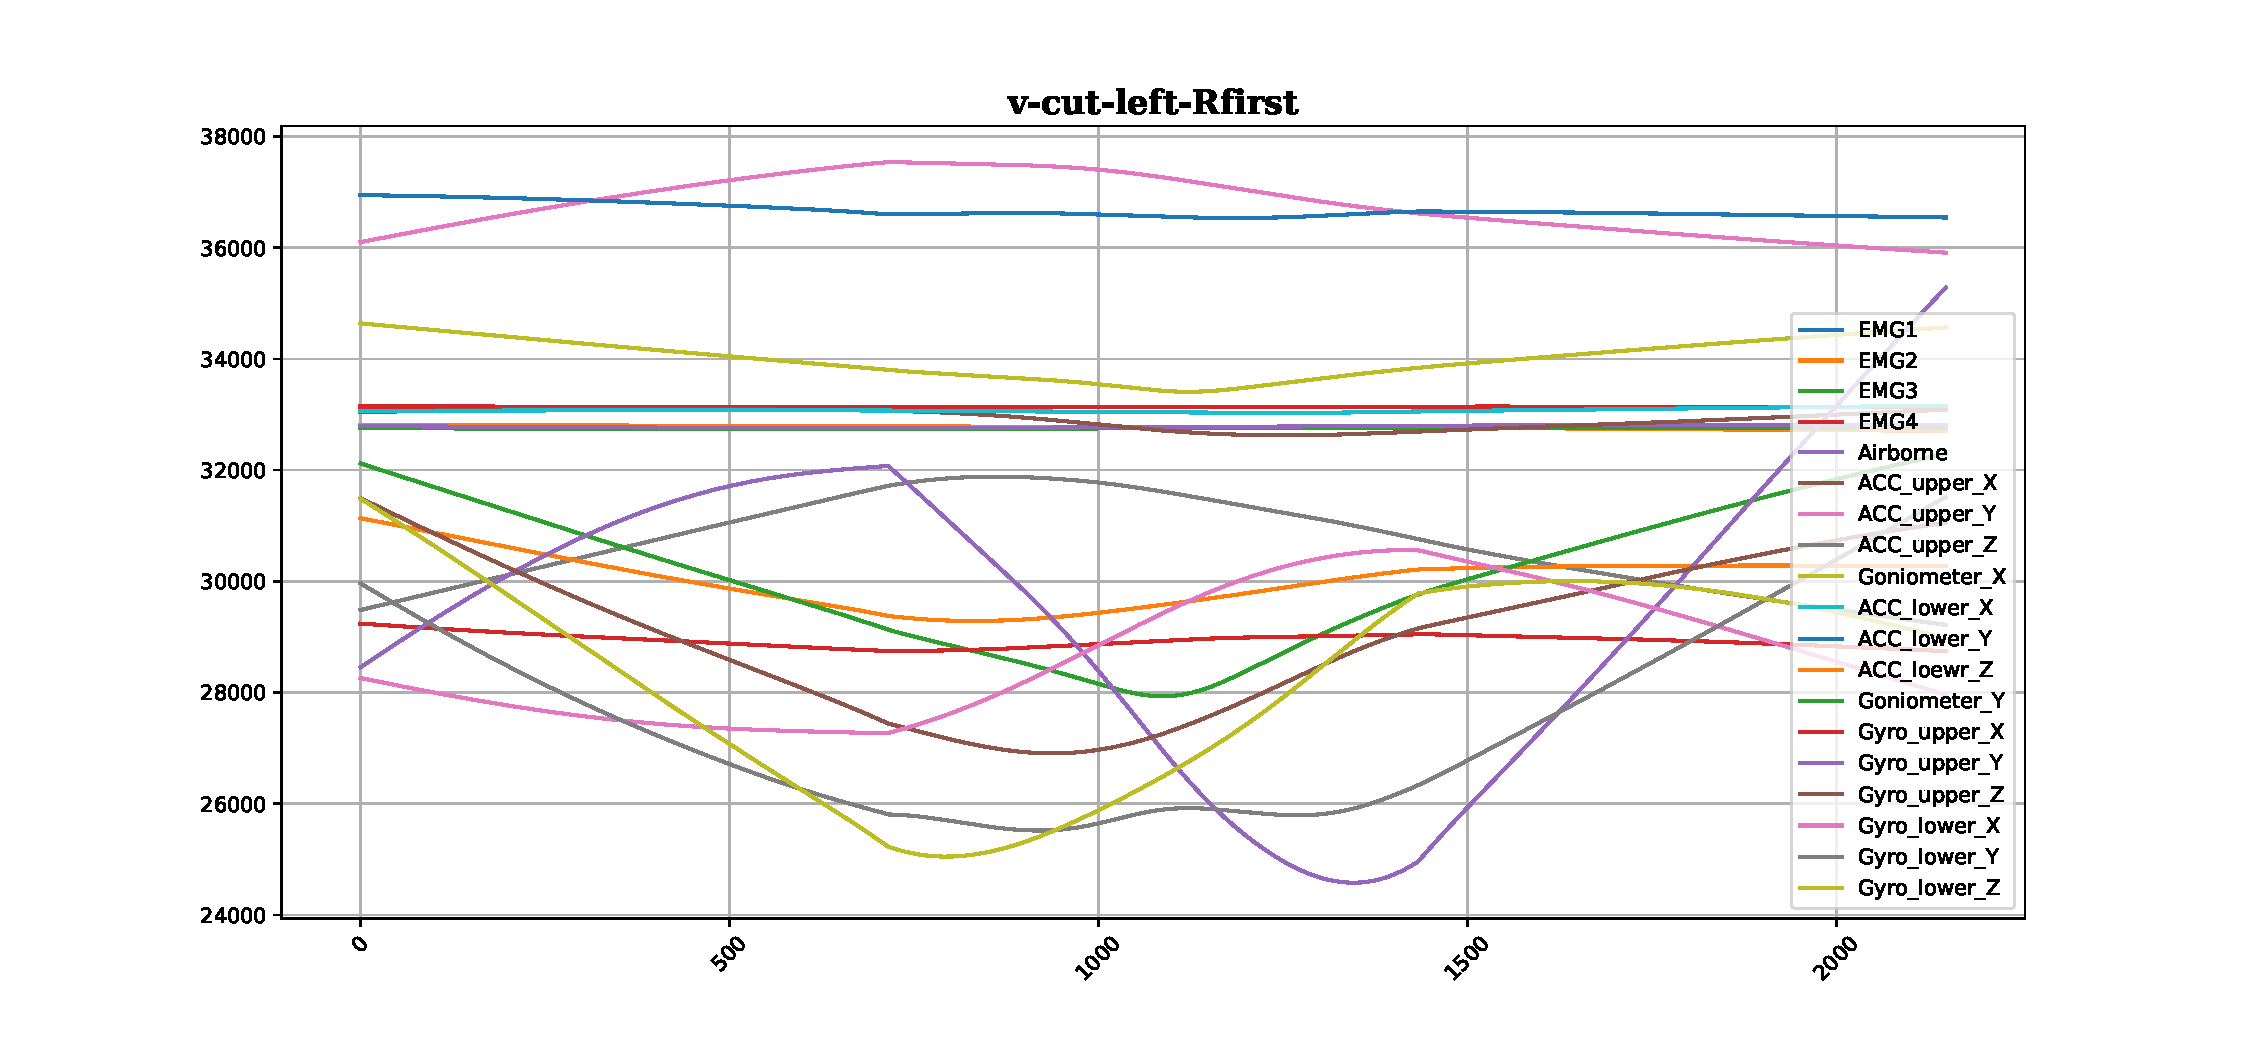
\includegraphics[width=\textwidth]{images/v-cut-left-Rfirst_example.pdf}
		\caption{v-cut-left-Rfirst}
	\end{minipage}
	\begin{minipage}[b]{0.31\textwidth}
		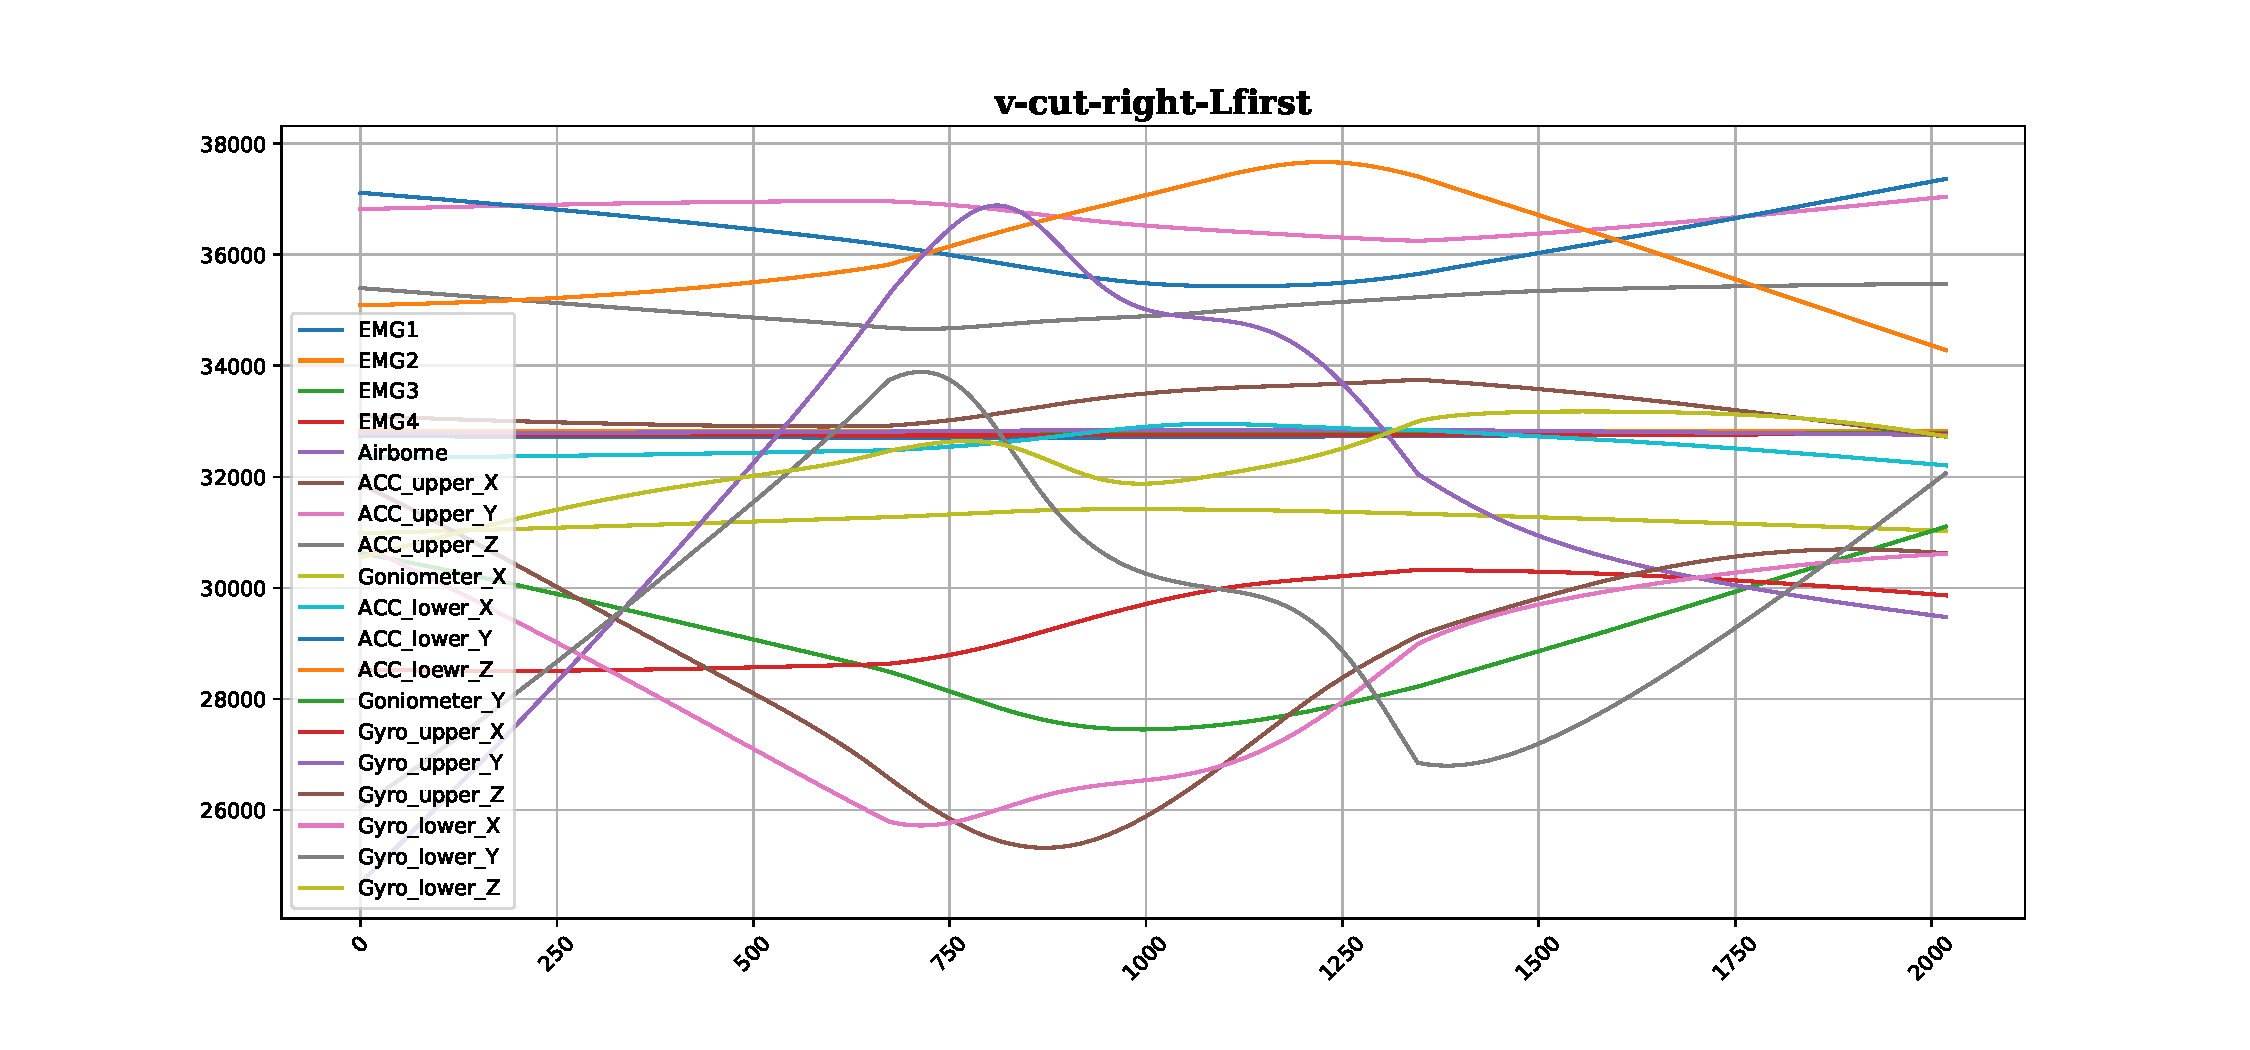
\includegraphics[width=\textwidth]{images/v-cut-right-Lfirst_example.pdf}
		\caption{v-cut-right-Lfirst}
	\end{minipage}
\end{figure}


\begin{figure}[!tbp]
	\begin{minipage}[b]{0.45\textwidth}
		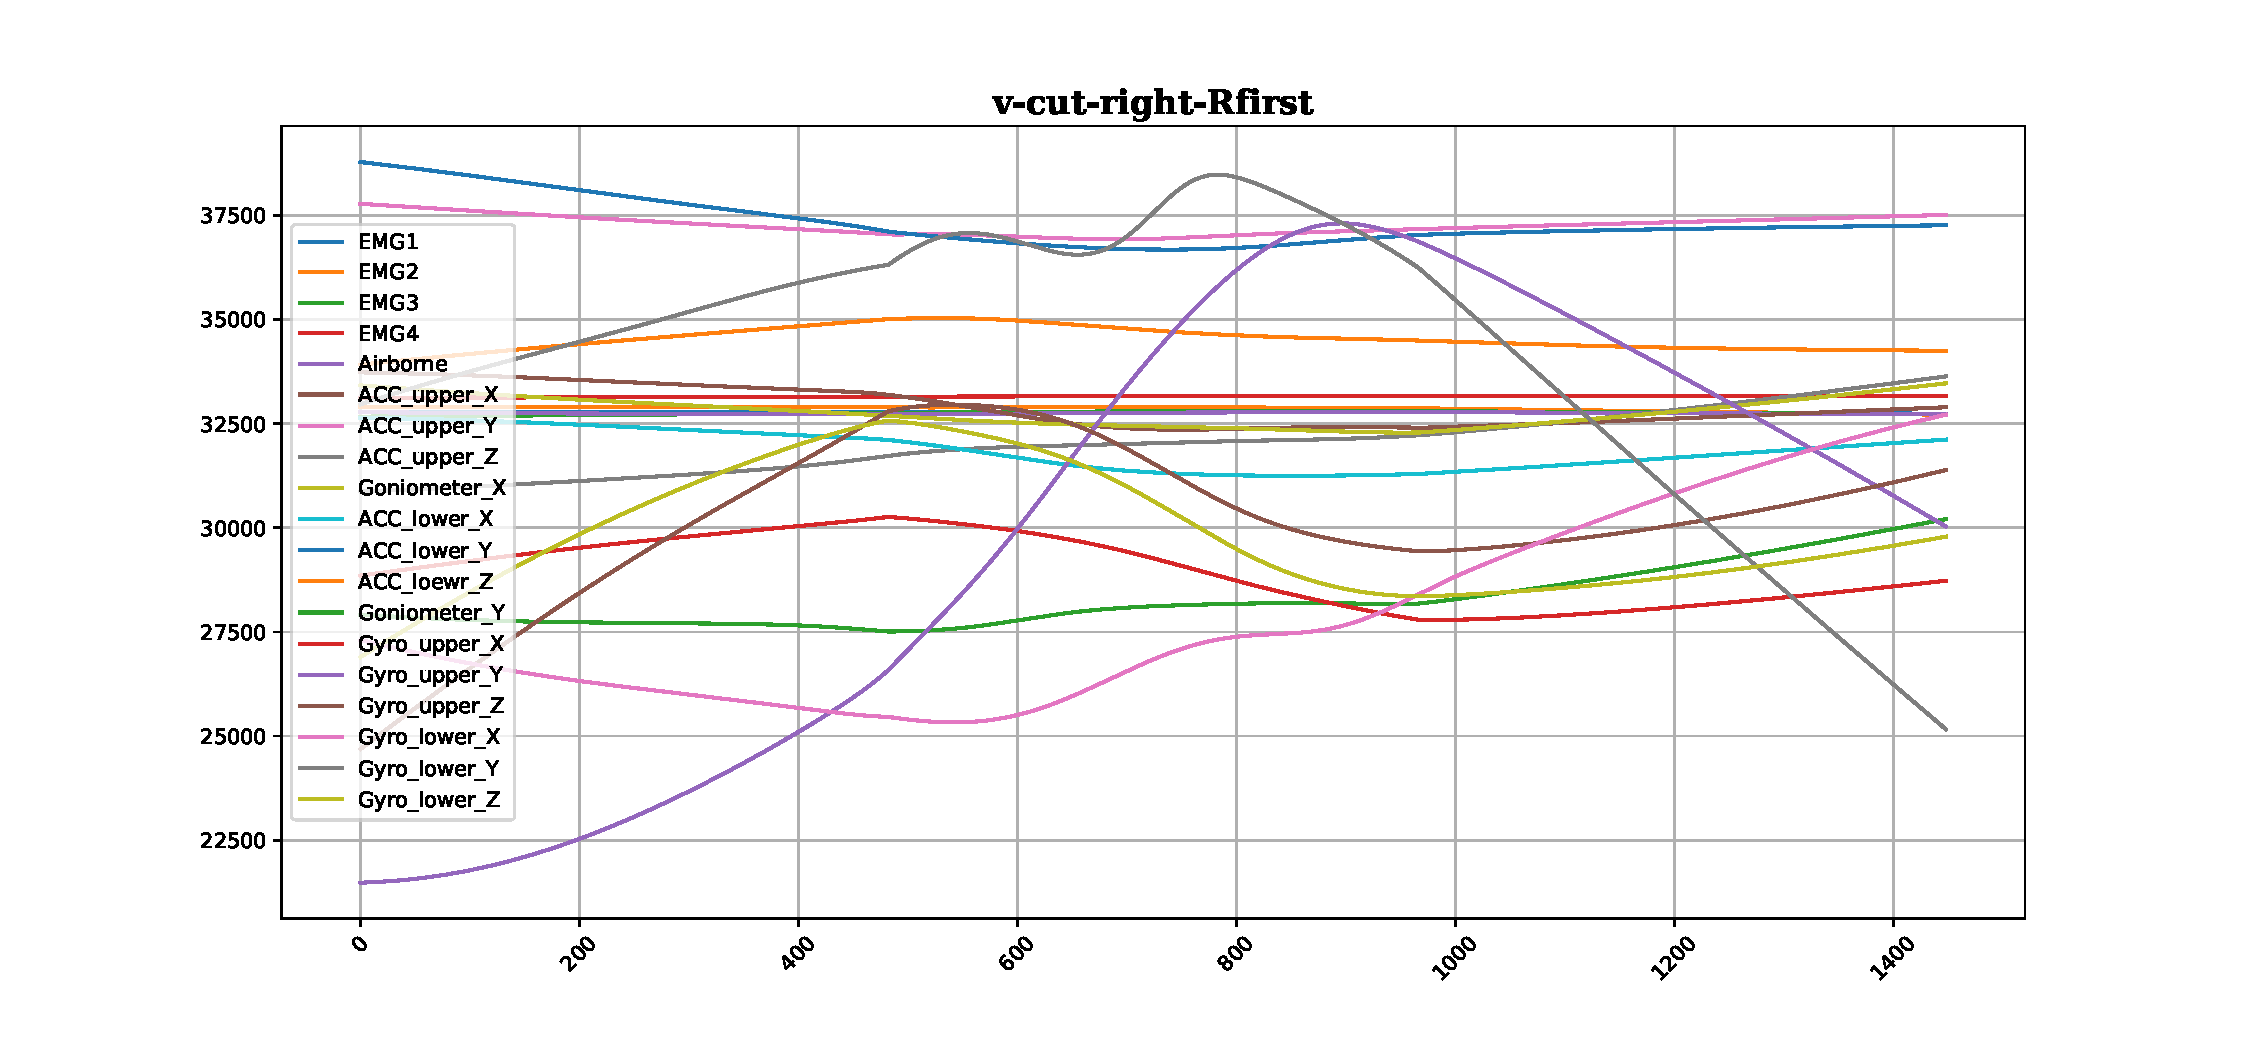
\includegraphics[width=\textwidth]{images/v-cut-right-Rfirst_example.pdf}
		\caption{v-cut-right-Rfirst}
	\end{minipage}
	\begin{minipage}[b]{0.45\textwidth}
		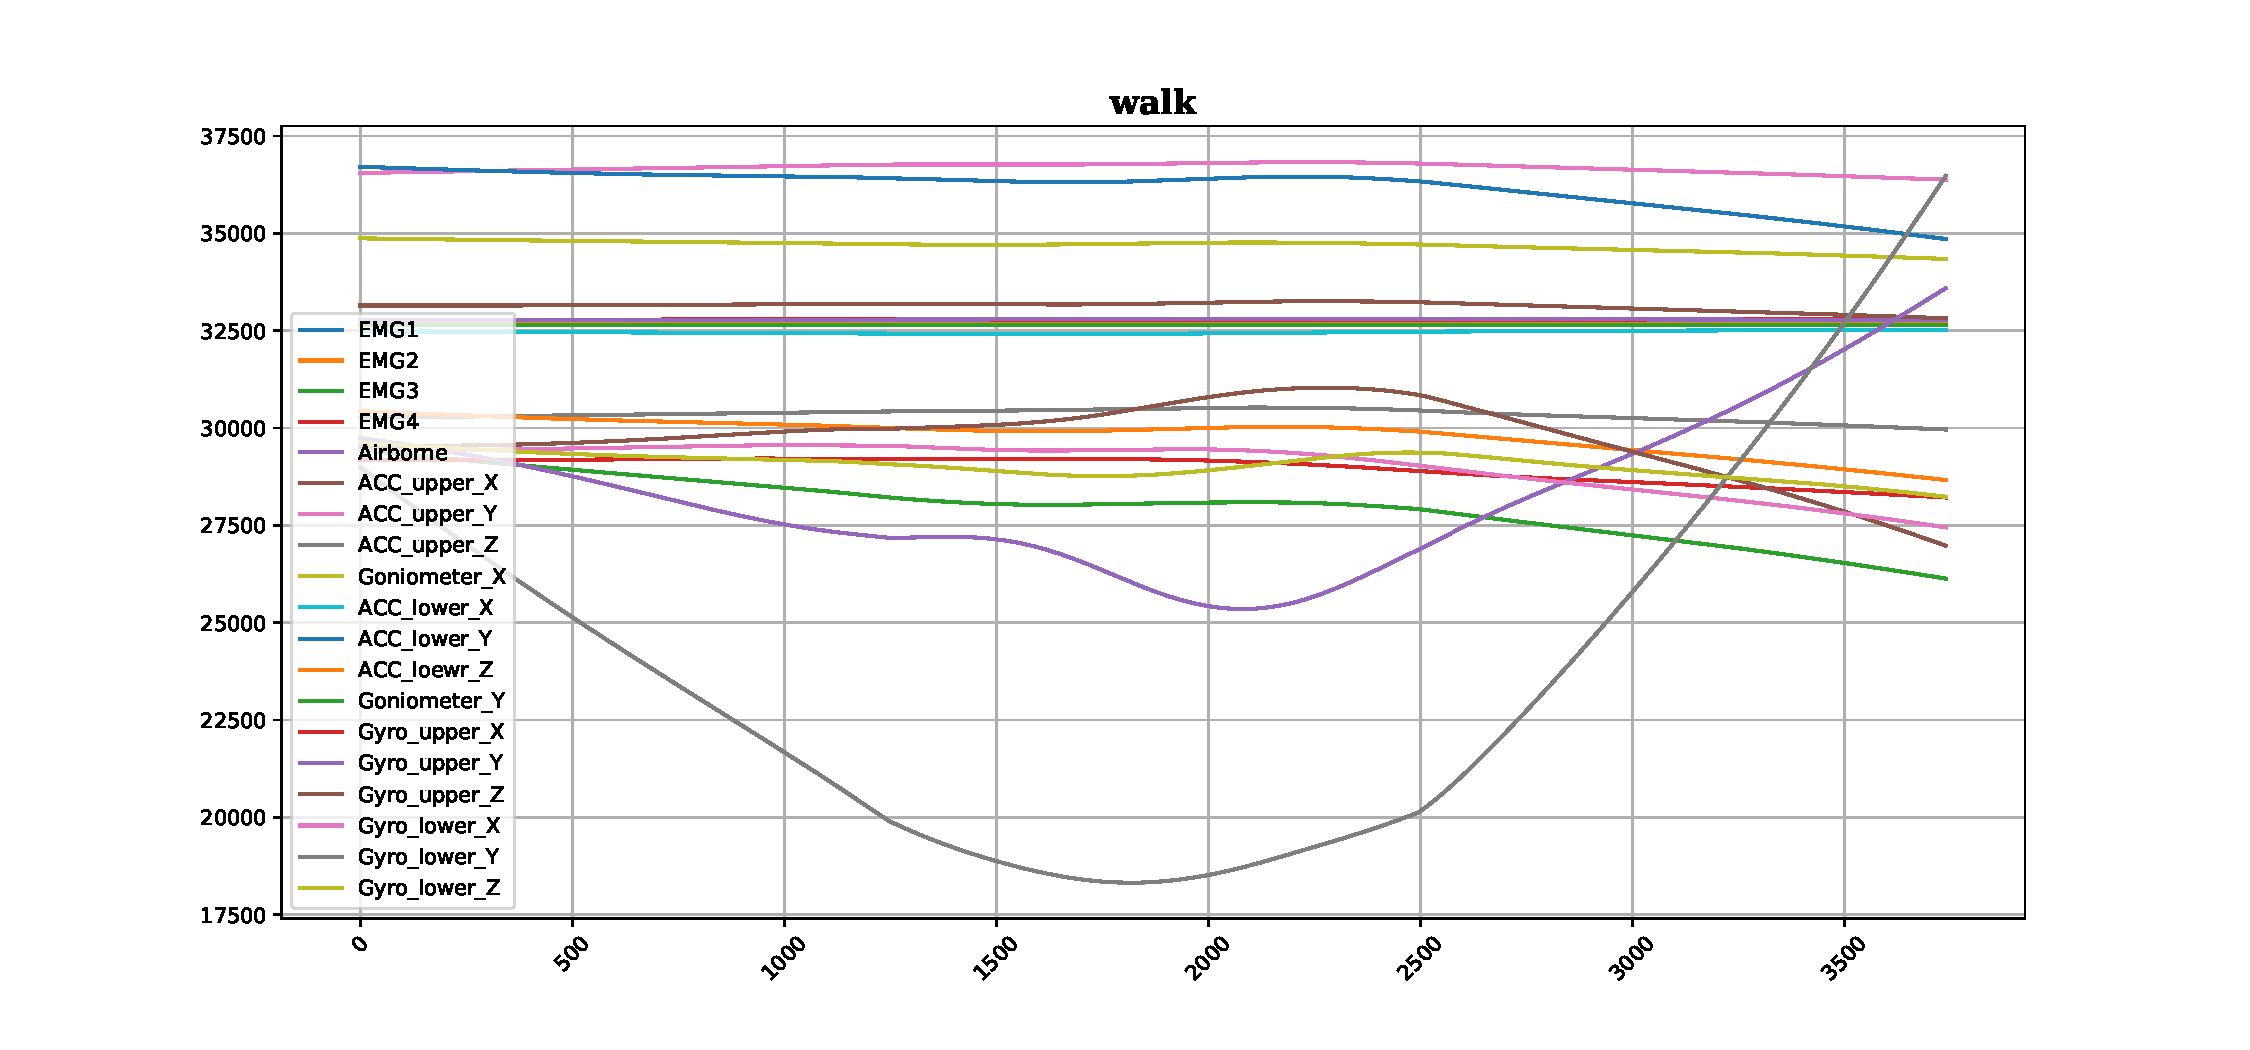
\includegraphics[width=\textwidth]{images/walk_example.pdf}
		\caption{walk}
		\label{sm22}
	\end{minipage}
\end{figure}



\section{Data Analysis}


\textit{Ralph i think it would be good if you explain here what you do when you implemented the "fully connected neuron network, like explain the parameters optimization and so on". that implementation will account for the neuron network at the end of the diagram in figure \ref{dig:p1}, report here also the score you got.}
By submitting both approaches to the challenge we observed that $\mathcal{P} (\Theta_{2})$ outperformed  $\mathcal{P}(\Theta_{1})$ so for this and the following sections we will focus our attention on  $\mathcal{P} (\Theta_{1})$

\section{Results and Discussions}




\begin{figure}[htpb!]
	\centering 
	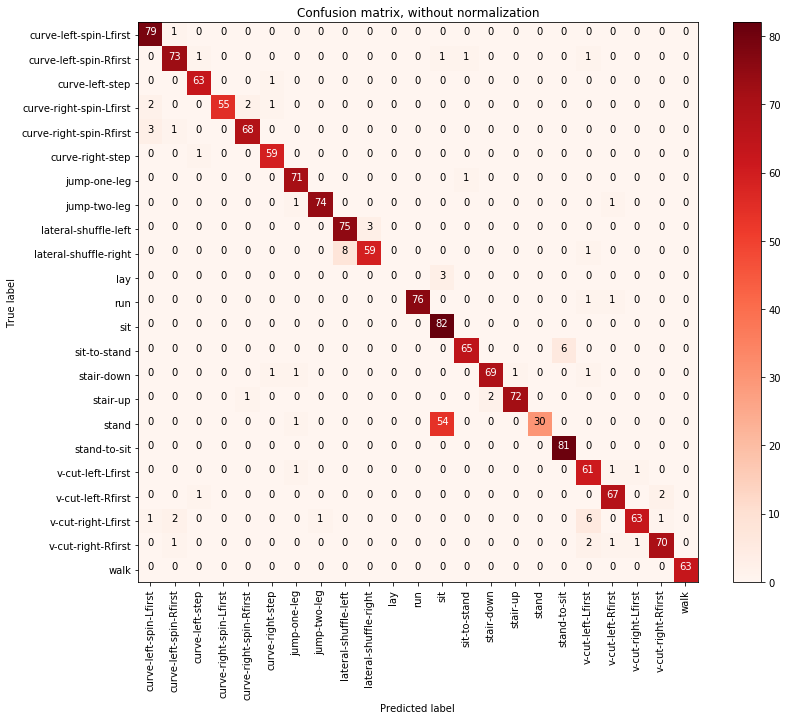
\includegraphics[width=\textwidth]{images/conf_ma.png}
	\caption{$\mathcal{P}(\Theta_{2})$  Confusion matrix on test data} 
	\label{fig:confusion} 
\end{figure}

\section{Conclusion}



\begin{thebibliography}{1}
\bibitem{1} 
Cleveland, W.S. (1979) “Robust Locally Weighted Regression and Smoothing Scatterplots”. Journal of the American Statistical Association 74 (368): 829-836.

\bibitem{2} 
Oraintara, S., Chen, Y. J., \& Nguyen, T. Q. (2002). Integer fast Fourier transform. IEEE Transactions on Signal Processing, 50(3), 607-618.

\end{thebibliography}

% ==============================================================================
% START: Methods, Results, Discussions, Conclusion
% ==============================================================================